% Main manuscript, Elsevier elsarticle (target: Computers in Biology and Medicine).
% Named build:       latexmk -pdf main.tex
% Blinded build:     latexmk -pdf manuscript_anonymised.tex   (defines \ANON before loading this file)
\documentclass[preprint,12pt,a4paper]{elsarticle}
\newif\ifanon
\ifdefined\ANON \anontrue \fi
\usepackage[T1]{fontenc}
\usepackage{newtxtext,newtxmath}
\usepackage[scaled=0.92]{helvet}
\usepackage{microtype}
\usepackage{amsmath}
\usepackage{booktabs,array,longtable,graphicx,float,placeins}
\usepackage{adjustbox}
\usepackage{enumitem}
\usepackage{xcolor}
\usepackage{url}
\usepackage{lineno}
\usepackage{tikz}
\usetikzlibrary{positioning,arrows.meta,calc,matrix}
\usepackage{pgfplots,pgfplotstable}
\pgfplotsset{compat=1.18}
\usepgfplotslibrary{groupplots}
\usepackage[colorlinks=true,linkcolor=blue!50!black,citecolor=blue!50!black,urlcolor=blue!50!black]{hyperref}
\biboptions{sort&compress}
\setlength{\parskip}{2pt}
% --- begin generated/numbers.tex
% auto-generated by experiments/report.py -- do not edit
\newcommand{\NMetabric}{2386}
\newcommand{\GThreeMetabric}{50.2}
\newcommand{\AgeMetabric}{61}
\newcommand{\NMsk}{1573}
\newcommand{\GThreeMsk}{67.6}
\newcommand{\AgeMsk}{52}
\newcommand{\NMbc}{207}
\newcommand{\GThreeMbc}{37.7}
\newcommand{\AgeMbc}{43}
\newcommand{\NSanger}{100}
\newcommand{\GThreeSanger}{51.0}
\newcommand{\AgeSanger}{55}
\newcommand{\NBroad}{59}
\newcommand{\GThreeBroad}{44.1}
\newcommand{\AgeBroad}{52}
\newcommand{\NBccrc}{63}
\newcommand{\GThreeBccrc}{88.9}
\newcommand{\AgeBccrc}{56}
\newcommand{\NTcga}{1072}
\newcommand{\GThreeTcga}{0.0}
\newcommand{\AgeTcga}{58}
\newcommand{\NDuke}{637}
\newcommand{\GThreeDuke}{32.5}
\newcommand{\AgeDuke}{52}
\newcommand{\NGradedTotal}{5025}
\newcommand{\NGradedCohorts}{7}
\newcommand{\NCohorts}{8}
\newcommand{\NAllTotal}{6097}
\newcommand{\NMetabricRecords}{2509}
\newcommand{\NMskSamples}{1918}
\newcommand{\NMskPatients}{1756}
\newcommand{\TauER}{-0.37}
\newcommand{\TauPR}{-0.31}
\newcommand{\TauHER}{+0.19}
\newcommand{\TauT}{+0.15}
\newcommand{\TauN}{+0.14}
\newcommand{\VHist}{0.18}
\newcommand{\RhoAge}{-0.12}
\newcommand{\NTests}{22}
\newcommand{\NSigTests}{20}
\newcommand{\BestIntModel}{Ordinal LR (prop. odds)}
\newcommand{\BestIntAuc}{0.725}
\newcommand{\BestIntAucLo}{0.709}
\newcommand{\BestIntAucHi}{0.743}
\newcommand{\MlrIntAuc}{0.725}
\newcommand{\OrdIntAuc}{0.725}
\newcommand{\XgbIntAuc}{0.723}
\newcommand{\KnnIntAuc}{0.715}
\newcommand{\IntAucSpread}{0.010}
\newcommand{\BestIntGThreeAuc}{0.752}
\newcommand{\IntAucMinR}{0.72}
\newcommand{\IntAucMaxR}{0.73}
\newcommand{\MlrIntFOne}{0.465}
\newcommand{\MajIntFOne}{0.223}
\newcommand{\MaxRepSd}{0.003}
\newcommand{\MaxDeltaInt}{0.008}
\newcommand{\MaxDeltaIntHi}{0.009}
\newcommand{\XgbDeltaInt}{+0.001}
\newcommand{\XgbDeltaIntLo}{-0.006}
\newcommand{\XgbDeltaIntHi}{+0.008}
\newcommand{\NSigBetterThanLr}{0}
\newcommand{\KnnDeltaInt}{-0.008}
\newcommand{\TabpfnStatus}{not run}
\newcommand{\TabpfnLimitation}{The pre-specified tabular foundation model (TabPFN) could not be run because its weights are distributed through a gated repository that was not reachable from the build environment; the code path is in place (\texttt{make tabpfn}). }
\newcommand{\BestExtModel}{Ordinal LR (prop. odds)}
\newcommand{\BestExtAuc}{0.713}
\newcommand{\BestExtAucLo}{0.688}
\newcommand{\BestExtAucHi}{0.737}
\newcommand{\MlrExtAuc}{0.710}
\newcommand{\XgbExtAuc}{0.711}
\newcommand{\MlrExtGThree}{0.727}
\newcommand{\NMskExt}{1573}
\newcommand{\CoreExtAucMin}{0.642}
\newcommand{\CoreExtAucMax}{0.797}
\newcommand{\LodoAucMin}{0.659}
\newcommand{\ExtAucMin}{0.64}
\newcommand{\ExtAucMax}{0.80}
\newcommand{\CoreMskMin}{0.64}
\newcommand{\CoreMskMax}{0.67}
\newcommand{\FullMskMin}{0.69}
\newcommand{\FullMskMax}{0.71}
\newcommand{\LodoAucMax}{0.778}
\newcommand{\NDukeExt}{637}
\newcommand{\MlrDukeAuc}{0.709}
\newcommand{\MlrDukeAucLo}{0.681}
\newcommand{\MlrDukeAucHi}{0.737}
\newcommand{\MlrDukeGThree}{0.779}
\newcommand{\FullDukeMin}{0.70}
\newcommand{\FullDukeMax}{0.72}
\newcommand{\MlrMskAucLo}{0.685}
\newcommand{\MlrMskAucHi}{0.734}
\newcommand{\NExtComparisons}{28}
\newcommand{\NExtSigBetter}{1}
\newcommand{\NExtSigWorse}{1}
\newcommand{\LeakMaxInfl}{+0.297}
\newcommand{\NpiHonest}{0.721}
\newcommand{\NpiLeaky}{0.972}
\newcommand{\SmoteHonestKnn}{0.652}
\newcommand{\SmoteLeakyKnn}{0.806}
\newcommand{\CompHonestDuke}{0.698}
\newcommand{\CompLeakyDuke}{0.995}
\newcommand{\CompHonest}{0.696}
\newcommand{\CompLeaky}{0.962}
\newcommand{\RecHonestKnn}{0.544}
\newcommand{\RecLeakyKnn}{0.579}
\newcommand{\CalIntMskRaw}{+0.99}
\newcommand{\CalSlopeMskRaw}{1.03}
\newcommand{\CalIntMskRec}{+0.00}
\newcommand{\CalSlopeInt}{1.00}
\newcommand{\CalSlopeIntXgb}{1.02}
\newcommand{\PrevMsk}{0.68}
\newcommand{\PredMsk}{0.47}
\newcommand{\CalIntDukeRaw}{-1.02}
\newcommand{\CalSlopeDukeRaw}{0.96}
\newcommand{\CalIntDukeRec}{+0.00}
\newcommand{\PrevDuke}{0.32}
\newcommand{\PredDuke}{0.52}
\newcommand{\CalSlopeMskXgb}{1.03}
\newcommand{\DcaLoInt}{0.26}
\newcommand{\DcaHiInt}{0.85}
\newcommand{\DcaLoExt}{0.63}
\newcommand{\DcaHiExt}{0.85}
\newcommand{\DcaLoDuke}{0.19}
\newcommand{\DcaHiDuke}{0.64}
\newcommand{\ShapAgree}{7 of 7}
\newcommand{\ShapTop}{ER positive}
\newcommand{\ShapSecond}{T category}
\newcommand{\OrER}{0.17}
\newcommand{\OrERlo}{0.12}
\newcommand{\OrERhi}{0.24}
\newcommand{\OrILC}{0.41}
\newcommand{\OrILClo}{0.28}
\newcommand{\OrILChi}{0.57}
\newcommand{\OrHer}{1.83}
\newcommand{\NOrdinal}{1800}
\newcommand{\RwGThreeMet}{60.9}
\newcommand{\RwGThreeMetLo}{58.5}
\newcommand{\RwGThreeMetHi}{63.0}
\newcommand{\ObsGThreeMet}{50.6}
\newcommand{\RwGOneMet}{6.2}
\newcommand{\RwGTwoMet}{32.9}
\newcommand{\EssMet}{1088}
\newcommand{\EssRedPct}{42}
\newcommand{\PredGThreeMet}{59.1}
\newcommand{\OverPredPP}{22}
\newcommand{\NRakedMet}{1861}
\newcommand{\AucUnwMet}{0.727}
\newcommand{\AucWMet}{0.790}
\newcommand{\RwGThreeMsk}{77.3}
\newcommand{\ObsGThreeMsk}{67.6}
\newcommand{\AucWMsk}{0.766}
\newcommand{\RwGThreeDuke}{42.1}
\newcommand{\ObsGThreeDuke}{32.5}
\newcommand{\RwGThreeMetB}{57.3}
\newcommand{\RwGThreeMetBLo}{54.6}
\newcommand{\RwGThreeMetBHi}{60.0}
\newcommand{\SaudiGThreeB}{48.8}
\newcommand{\PoolGThree}{44.7}
\newcommand{\PoolGThreeLo}{37.2}
\newcommand{\PoolGThreeHi}{52.5}
\newcommand{\PoolK}{3}
\newcommand{\PoolN}{908}
\newcommand{\AgeSensMin}{60.5}
\newcommand{\AgeSensMax}{61.3}
\newcommand{\AgeSensLo}{40}
\newcommand{\AgeSensHi}{60}
\newcommand{\RwGThreeAllMin}{35.9}
\newcommand{\ShiftMin}{+9.6}
\newcommand{\ShiftMax}{+10.3}
\newcommand{\ObsGThreeMin}{32.5}
\newcommand{\ObsGThreeMax}{67.6}
\newcommand{\RwGThreeKMin}{42.1}
\newcommand{\RwGThreeKMax}{77.3}
\newcommand{\SaudiGThreeA}{36.7}
\newcommand{\RwGThreeAllMax}{77.3}
\newcommand{\MIDiffMax}{0.003}
\newcommand{\MIMlrAuc}{0.724}
\newcommand{\MIXgbAuc}{0.726}
\newcommand{\NComplete}{1800}
\newcommand{\CCMlrAuc}{0.729}
\newcommand{\MIm}{20}
\newcommand{\DukeClinAuc}{0.694}
\newcommand{\DukeClinAucLo}{0.663}
\newcommand{\DukeClinAucHi}{0.727}
\newcommand{\DukeClinGThree}{0.769}
\newcommand{\DukeRadAuc}{0.608}
\newcommand{\DukeRadAucLo}{0.575}
\newcommand{\DukeRadAucHi}{0.645}
\newcommand{\DukeRadGThree}{0.667}
\newcommand{\DukeFusAuc}{0.648}
\newcommand{\DukeFusAucLo}{0.618}
\newcommand{\DukeFusAucHi}{0.685}
\newcommand{\DukeFusGThree}{0.731}
\newcommand{\DukeRadDelta}{-0.085}
\newcommand{\DukeRadDeltaLo}{-0.126}
\newcommand{\DukeRadDeltaHi}{-0.045}
\newcommand{\DukeFusDelta}{-0.045}
\newcommand{\DukeFusDeltaLo}{-0.077}
\newcommand{\DukeFusDeltaHi}{-0.011}
\newcommand{\NDukeRad}{637}
\newcommand{\SSRequired}{4477}
\newcommand{\SSAvailable}{2386}
\newcommand{\SSParams}{10}
\newcommand{\SSMet}{not met}
\newcommand{\LjBest}{0.636}
\newcommand{\NLj}{286}
\newcommand{\Repeats}{10}
\newcommand{\Folds}{5}
\newcommand{\InnerFolds}{3}
\newcommand{\Boot}{2000}
\newcommand{\Seed}{20261017}
\newcommand{\TransportBoot}{500}
\newcommand{\RadRepeats}{10}
% --- end generated/numbers.tex

% --- begin figures/pgfstyle.tex
% Shared pgfplots style. Data come from generated/data/*.csv (written by experiments/report.py).
\definecolor{cA}{HTML}{2A78D6}\definecolor{cB}{HTML}{EB6834}\definecolor{cC}{HTML}{1BAF7A}\definecolor{cD}{HTML}{6250D6}
\definecolor{gI}{HTML}{B9D3F2}\definecolor{gII}{HTML}{5D98DE}\definecolor{gIII}{HTML}{174F94}
\definecolor{inkb}{HTML}{52514E}\definecolor{gridc}{HTML}{E4E3DF}
\pgfplotstableset{col sep=semicolon}
\pgfplotsset{
  table/col sep=semicolon,
  bcbase/.style={font=\sffamily\scriptsize, axis line style={inkb}, tick style={inkb},
    major grid style={gridc}, tick align=outside, axis x line*=bottom, axis y line*=left,
    legend style={draw=none, fill=none, font=\sffamily\scriptsize}, legend cell align=left},
  dotci/.style={only marks, mark=*, mark size=1.6pt, #1, error bars/.cd, x dir=both, x explicit,
    error bar style={#1, line width=1pt}, error mark=none},
}
\newcommand{\gdata}[1]{generated/data/#1.csv}
% --- end figures/pgfstyle.tex

\newcommand{\tabfit}[1]{\resizebox{\linewidth}{!}{#1}}
% repository link: replace with the anonymous mirror for review and the public URL/DOI after acceptance
\newcommand{\CodeURL}{\url{https://anonymous.4open.science/r/bc-grade-opendata}}
\journal{Computers in Biology and Medicine}

\begin{document}
\ifanon\linenumbers\fi

\begin{frontmatter}
\title{How much of breast cancer grade is in the routine record? A leakage-audited,
multi-cohort open-data prediction study with MRI radiomics and transport to Saudi case-mix}

\ifanon
\author{[Author details removed for double-anonymised review]}
\else
\IfFileExists{authors.tex}{% --- begin authors.tex
% Author block (named build). Replaced by authors_placeholder.tex in the review repository.
\author[uhb]{Aminat Abiola Ajibola\corref{cor1}}
\ead{aajibola@uhb.edu.sa}
\cortext[cor1]{Corresponding author. Tel.: +966 550047554.}
\affiliation[uhb]{organization={College of Computer Science and Engineering, University of Hafr Al-Batin},
  state={Eastern Province}, country={Kingdom of Saudi Arabia}}
% --- end authors.tex
}{% --- begin authors_placeholder.tex
% Placeholder used in the public/anonymous repository; the submission files carry the real author block.
\author{[Author details withheld for double-anonymised review]}
% --- end authors_placeholder.tex
}
\fi

% --- begin sections/abstract.tex
\begin{abstract}
\textbf{Background:} Nottingham grade guides breast cancer management but is a tissue-based,
moderately reproducible judgement. How much of it routine variables carry, whether such models
transport, and what they imply for Saudi patients is unknown.
\textbf{Methods:} We harmonised \NGradedTotal{} grade-labelled invasive cancers from \NGradedCohorts{}
open cohorts. Seven models, from a prevalence baseline to gradient boosting, were developed in
METABRIC (\NMetabric{} patients) with nested cross-validation, compared with logistic regression by
paired bootstrap, and validated, frozen, in five external cohorts and by leave-one-dataset-out. We
report discrimination, calibration, decision curves, a leakage audit, an MRI-radiomics extension and
re-weighting to published Saudi case-mix (TRIPOD+AI).
\textbf{Results:} Internal macro-AUC was \IntAucMinR--\IntAucMaxR{} for every learned model; XGBoost
minus logistic regression was \XgbDeltaInt{} (95\% CI \XgbDeltaIntLo{} to \XgbDeltaIntHi). External
macro-AUCs were \FullMskMin--\FullMskMax{} (MSK-2018) and \FullDukeMin--\FullDukeMax{} (Duke).
Calibration slopes stayed near one, but grade-3 calibration-in-the-large failed in opposite
directions (intercepts \CalIntMskRaw{} and \CalIntDukeRaw) and was corrected by an intercept update.
Leaky protocols inflated macro-AUC by up to \LeakMaxInfl. Adding 529 DCE-MRI radiomic features did
not help ($\Delta$ \DukeFusDelta, \DukeFusDeltaLo{} to \DukeFusDeltaHi). Saudi case-mix raised
each cohort's grade-3 share by \ShiftMin{} to \ShiftMax{} points, yet a METABRIC-developed model would
predict \PredGThreeMet\% grade~3 against \SaudiGThreeA\% published.
\textbf{Conclusions:} Routine variables carry moderate, transportable information about grade;
logistic regression suffices and calibration must be updated locally. Western-developed models would
over-predict high-grade disease in Saudi patients.
\end{abstract}
% --- end sections/abstract.tex


\begin{keyword}
breast cancer \sep histological grade \sep clinical prediction model \sep external validation \sep
calibration \sep data leakage \sep radiomics \sep transportability \sep Saudi Arabia \sep TRIPOD+AI
\end{keyword}
\end{frontmatter}

% --- begin sections/introduction.tex
\section{Introduction}\label{sec:intro}

\paragraph{Grade matters, but it is assigned late and inconsistently}
Nottingham (Elston--Ellis) histological grade combines tubule formation, nuclear pleomorphism and
mitotic count into a three-level score that remains one of the strongest independent prognostic
factors in invasive breast cancer~\citep{elston1991grade,rakha2008nhg,rakha2010grade}. It is,
however, a tissue-based judgement made after biopsy or excision, and it is only moderately
reproducible: agreement between departments and pathologists is typically in the $\kappa$ range
0.5--0.7~\citep{boiesen2000grading,longacre2006interobserver}, grading proportions vary
significantly between and within laboratories in national data~\citep{vandooijeweert2020variation},
and the intermediate grade~2, which accounts for a large share of tumours, is prognostically
heterogeneous~\citep{sotiriou2006ggi,vandooijeweert2022grading}. These facts motivate a simple but
rarely answered question: \emph{how much of a tumour's grade is already carried by the routinely
recorded clinicopathological variables}---age, menopausal status, ER, PR and HER2 status,
histological type, tumour size and nodal status? A credible answer would serve as a baseline against
which image-based grade predictors are judged, as a tool for imputing grade where registry records
lack it, and as a quality-assurance signal when an assigned grade is improbable given the rest of the
record.

\paragraph{Computational grading has moved to images without a tabular baseline}
Recent work predicts grade from whole-slide images with deep learning and pathology foundation
models~\citep{wang2022deepgrade,kim2025grade,chen2024uni} and from dynamic contrast-enhanced MRI
radiomics~\citep{wang2022duke,wang2026dcemrigrade}. We found no study that quantified, on open
multi-cohort data, how well the routine clinicopathological record alone predicts three-level grade,
how such a model behaves outside its development population, or how much of the reported performance
in this area could be produced by analytic leakage. Leakage---information about the outcome reaching
the model through predictors that encode it, through preprocessing fitted before data splitting, or
through repeated records of the same patient---is a recognised cause of irreproducible machine-learning
results in medicine~\citep{kapoor2023leakage,varoquaux2022failures,rosenblatt2024leakage}. Grade is
unusually exposed to it, because widely shared datasets carry composite indices (the Nottingham
Prognostic Index) and component scores that contain grade by construction. Separately, systematic
reviews show that flexible learners seldom outperform regression for clinical
prediction~\citep{christodoulou2019lr}, that calibration is the most frequently neglected property
of prediction models~\citep{vancalster2019calibration}, and that external validation and reporting
should follow TRIPOD+AI~\citep{collins2024tripodai,collins2024evalpart1,riley2024evalpart2}.

\paragraph{The Saudi and Gulf context, and the problem of transport}
Breast cancer is the most common cancer among Saudi women; its age-standardised incidence in Saudi
females rose from 11.8 to 29.7 per 100{,}000 between 2001 and 2017, when it accounted for 30.9\% of
female cancers, with a median age at diagnosis of about 51 years~\citep{basudan2022registry}.
Patients in Arab countries present younger and more often with hormone-receptor-negative and
HER2-positive disease than patients in Western screening
cohorts~\citep{najjar2010arab,chouchane2013arab,elkum2007young,altamimi2010saudi,kussaibi2021saudi}.
Yet no grade-labelled patient-level dataset from the region is openly available, and local analyses
are typically based on single-centre hospital records that cannot be shared or independently
checked~\citep{kussaibi2021saudi,durrani2025healthcare}. A model developed elsewhere can only be used in a new population if it
\emph{transports}: case-mix differences can change both its discrimination and, above all, its
calibration~\citep{debray2015framework,steingrimsson2023transport,riley2016bigdata}. Whether Western
grade models transport to Saudi case-mix is therefore an open and practically important question
that can be approached, without patient data, by re-weighting open cohorts to published Saudi
aggregates.

\paragraph{Design principles}
Clinicopathological analyses of grade are prone to avoidable errors: correlation coefficients
computed on arbitrary codes of nominal categories, causal readings of cross-sectional associations,
in-situ carcinoma counted as invasive disease, lobular carcinoma merged with ductal carcinoma, and
validation designs in which imputation, resampling or repeated records let information cross from
test to training data~\citep{kapoor2023leakage,varoquaux2022failures}. We therefore fixed the
harmonisation rules, feature sets, models, metrics and expected directions of effect before running
the experiments, and used only openly downloadable cohorts, so that every number in this paper can be
regenerated by a reviewer.

\paragraph{Contributions}
\begin{enumerate}[leftmargin=*,itemsep=1pt,topsep=2pt]
\item An open, checksummed, harmonised common data model of \NGradedTotal{} grade-labelled invasive
breast cancers from \NGradedCohorts{} cohorts in three continents, with explicit rules that prevent the
in-situ, histology and duplication errors described above (Figure~\ref{fig:framework}).
\item A TRIPOD+AI-compliant model ladder from a prevalence baseline to gradient boosting, with nested
cross-validation, multiple imputation, paired comparisons against logistic regression, external
validation in two full-feature and three core-feature cohorts, leave-one-dataset-out validation,
calibration, model updating and decision curves.
\item A leakage audit that quantifies, on the same data and models, how much four common shortcuts
inflate apparent discrimination.
\item An imaging extension in the Duke breast MRI cohort that asks whether 529 DCE-MRI radiomic
features add to the routine clinical record.
\item A case-mix transport analysis that re-weights open cohorts to published Saudi hospital series
and shows what Western-developed grade models would imply for Saudi patients.
\end{enumerate}
% --- end sections/introduction.tex

% --- begin sections/methods.tex
\section{Methods}\label{sec:methods}

\subsection{Design, reporting and framework}
This is a secondary analysis of de-identified, publicly released data. The prediction component is
reported according to TRIPOD+AI~\citep{collins2024tripodai} and the descriptive component according
to STROBE~\citep{vonelm2007strobe}; the full TRIPOD+AI checklist is in Supplementary
Table~\ref{tab:tripod}. Figure~\ref{fig:framework} summarises the framework: open sources are
harmonised to a common data model (lane A); the model is developed and validated (lane B); and the
results are stress-tested by a leakage audit, a plausibility check, an imaging extension and a
transport analysis (lane C). Feature sets, model ladder, metrics, expected directions of effect and
raking targets were fixed in \texttt{configs/experiment.yaml} before the experiments were run (seed
\Seed). Every table, figure and in-text number is produced by code from the results files; none is
typed by hand.

\begin{figure*}[t]\centering
\resizebox{\linewidth}{!}{% --- begin figures/fig_framework.tex
% Figure 1 -- study framework (three lanes). Counts are macros from generated/numbers.tex.
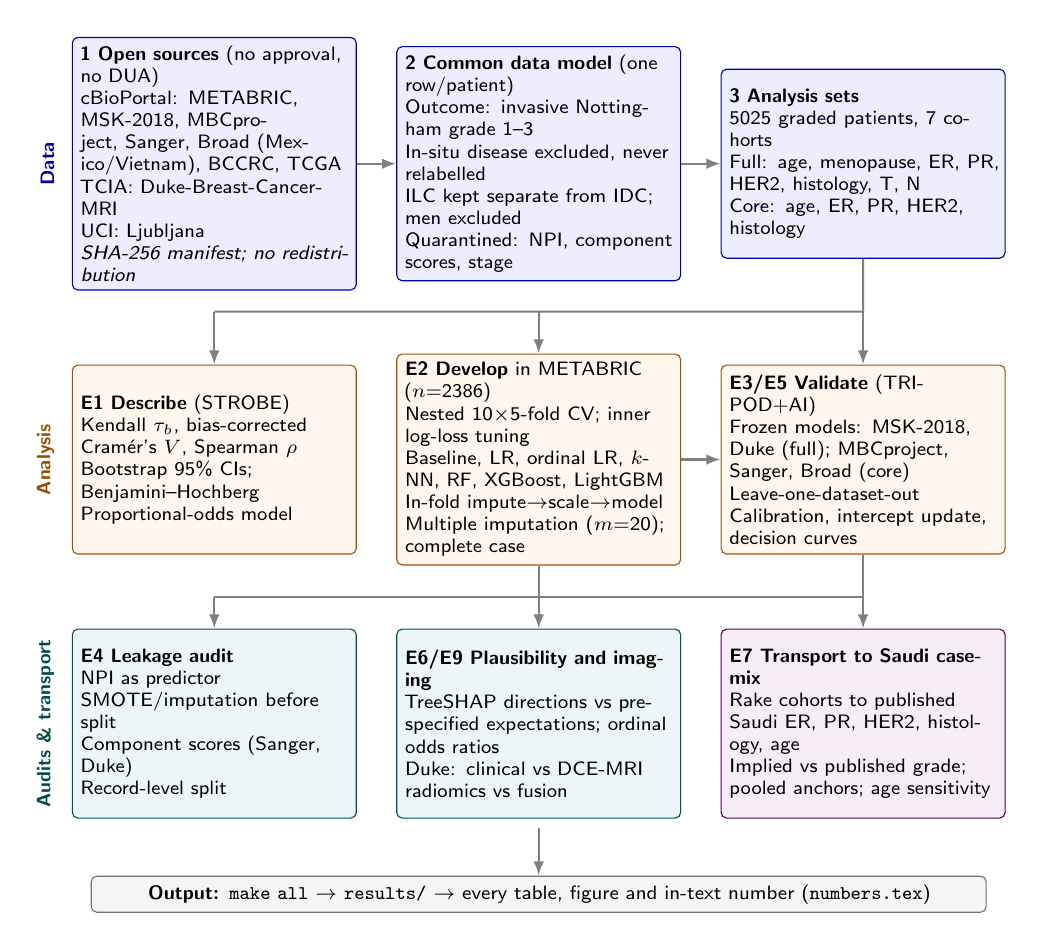
\begin{tikzpicture}[
  font=\sffamily\scriptsize,
  box/.style={draw=#1!65!black, fill=#1!7, rounded corners=2pt, align=left, inner sep=3pt,
              text width=0.28\linewidth, minimum height=24mm},
  lane/.style={font=\sffamily\scriptsize\bfseries, text=#1!60!black, rotate=90, anchor=south},
  arr/.style={-{Latex[length=1.8mm]}, thick, draw=black!50},
  bus/.style={thick, draw=black!50},
]
\matrix (m) [row sep=8mm, column sep=5mm, ampersand replacement=\&] {
\node[box=blue] (src) {\textbf{1 Open sources} (no approval, no DUA)\\
  cBioPortal: METABRIC, MSK-2018, MBCproject, Sanger, Broad (Mexico/Vietnam), BCCRC, TCGA\\
  TCIA: Duke-Breast-Cancer-MRI\\
  UCI: Ljubljana\\
  \emph{SHA-256 manifest; no redistribution}}; \&
\node[box=blue] (cdm) {\textbf{2 Common data model} (one row/patient)\\
  Outcome: invasive Nottingham grade 1--3\\
  In-situ disease excluded, never relabelled\\
  ILC kept separate from IDC; men excluded\\
  Quarantined: NPI, component scores, stage}; \&
\node[box=blue] (fs) {\textbf{3 Analysis sets}\\
  \NGradedTotal{} graded patients, \NGradedCohorts{} cohorts\\
  Full: age, menopause, ER, PR, HER2, histology, T, N\\
  Core: age, ER, PR, HER2, histology}; \\
\node[box=orange] (e1) {\textbf{E1 Describe} (STROBE)\\
  Kendall $\tau_b$, bias-corrected Cram\'er's $V$, Spearman $\rho$\\
  Bootstrap 95\% CIs; Benjamini--Hochberg\\
  Proportional-odds model}; \&
\node[box=orange] (e2) {\textbf{E2 Develop} in METABRIC ($n$=\NMetabric)\\
  Nested \Repeats$\times$\Folds-fold CV; inner log-loss tuning\\
  Baseline, LR, ordinal LR, $k$-NN, RF, XGBoost, LightGBM\\
  In-fold impute$\to$scale$\to$model\\
  Multiple imputation ($m$=\MIm); complete case}; \&
\node[box=orange] (e3) {\textbf{E3/E5 Validate} (TRIPOD+AI)\\
  Frozen models: MSK-2018, Duke (full); MBCproject, Sanger, Broad (core)\\
  Leave-one-dataset-out\\
  Calibration, intercept update, decision curves}; \\
\node[box=teal] (e4) {\textbf{E4 Leakage audit}\\
  NPI as predictor\\ SMOTE/imputation before split\\ Component scores (Sanger, Duke)\\ Record-level split}; \&
\node[box=teal] (e6) {\textbf{E6/E9 Plausibility and imaging}\\
  TreeSHAP directions vs pre-specified expectations; ordinal odds ratios\\
  Duke: clinical vs DCE-MRI radiomics vs fusion}; \&
\node[box=violet] (e7) {\textbf{E7 Transport to Saudi case-mix}\\
  Rake cohorts to published Saudi ER, PR, HER2, histology, age\\
  Implied vs published grade; pooled anchors; age sensitivity}; \\
};
\node[draw=black!55, fill=black!4, rounded corners=2pt, anchor=north, inner sep=3pt, align=center,
      text width=0.92\linewidth] (out) at ([yshift=-6mm]m.south)
  {\textbf{Output:} \texttt{make all} $\to$ \texttt{results/} $\to$ every table, figure and in-text number (\texttt{numbers.tex})};
\draw[arr] (src) -- (cdm); \draw[arr] (cdm) -- (fs);
% bus from data lane to analysis lane
\coordinate (b1) at ($(fs.south)!0.5!(e3.north)$);
\draw[bus] (fs.south) -- (b1) -- (b1 -| e1.north);
\foreach \n in {e1,e2,e3} \draw[arr] (b1 -| \n.north) -- (\n.north);
\draw[arr] (e2) -- (e3);
% bus from analysis lane to audit lane
\coordinate (b2) at ($(e2.south)!0.5!(e6.north)$);
\draw[bus] (e2.south) -- (b2); \draw[bus] (b2 -| e4.north) -- (b2 -| e7.north);
\draw[bus] (e3.south) -- (b2 -| e3.south);
\foreach \n in {e4,e6,e7} \draw[arr] (b2 -| \n.north) -- (\n.north);
\draw[arr] (m.south) -- (out.north);
\node[lane=blue]   at ([xshift=-1mm]src.west) {Data};
\node[lane=orange] at ([xshift=-1mm]e1.west)  {Analysis};
\node[lane=teal]   at ([xshift=-1mm]e4.west)  {Audits \& transport};
\end{tikzpicture}
% --- end figures/fig_framework.tex
}
\caption{Study framework. \textbf{A}, open data are downloaded with checksums and mapped to one row
per patient under four harmonisation rules; variables that encode grade are quarantined. \textbf{B},
associations are described with scale-appropriate statistics; models are developed in METABRIC with
nested cross-validation and validated, frozen, in five external cohorts and by leave-one-dataset-out.
\textbf{C}, the results are audited for leakage and clinical plausibility, extended with MRI
radiomics in the Duke cohort, and transported to published Saudi case-mix. E1--E10 are the
experiment stages in the repository.}\label{fig:framework}
\end{figure*}

\subsection{Data sources}
Tabular data were obtained without registration from the cBioPortal data
hub~\citep{cerami2012cbio,gao2013cbio}, The Cancer Imaging Archive and the UCI Machine Learning
Repository. A download script records SHA-256 checksums so that silent upstream changes are
detectable. Cohorts and roles were:
\begin{itemize}[leftmargin=*,itemsep=1pt,topsep=2pt]
\item \textbf{METABRIC} (UK/Canada; development)~\citep{curtis2012metabric,pereira2016metabric}:
surgical cohort with Nottingham grade, tumour size (mm), positive-node count, receptors and inferred
menopausal state.
\item \textbf{MSK-2018} (USA; external, full feature set)~\citep{razavi2018msk}: patients sequenced
at Memorial Sloan Kettering, enriched for advanced hormone-receptor-positive disease, with
diagnosis-time grade, T and N category, receptors and menopausal status.
\item \textbf{Duke-Breast-Cancer-MRI} (USA; external, full feature set; imaging
extension)~\citep{saha2018duke}: 922 patients with invasive cancer imaged at Duke University
Hospital (2000--2014), with Nottingham grade and its component scores, receptors, T and N category,
menopausal status and 529 pre-computed DCE-MRI features (CC BY-NC 4.0; files obtained from a
checksummed public mirror of the TCIA release).
\item \textbf{MBCproject} (USA/Canada; external, core features)~\citep{mbcproject2022,jain2023mbcproject}:
patient-partnered metastatic cohort with abstracted diagnosis-time records; age in five-year bands.
\item \textbf{Sanger} (UK/Europe; external, core)~\citep{stephens2012sanger}: 100 primary tumours
with grade and the three Nottingham component scores.
\item \textbf{Broad} (Mexico and Vietnam; external, core)~\citep{banerji2012broad}: the only open
grade-labelled cohort from low- and middle-income countries we identified.
\item \textbf{BCCRC} (Canada; triple-negative; descriptive)~\citep{shah2012bccrc} and
\textbf{TCGA-BRCA} (USA; descriptive, no structured grade)~\citep{tcga2012brca}.
\item \textbf{Ljubljana} (Slovenia; sensitivity)~\citep{zwitter1988ljubljana}: \NLj{} patients with
``degree of malignancy'' 1--3 and binned covariates.
\end{itemize}
No openly downloadable, grade-labelled patient-level cohort from Saudi Arabia or the Gulf was
identified; Saudi relevance enters through published aggregates (Section~\ref{sec:transport}).

\subsection{Harmonisation to a common data model}
Each source was mapped to one row per patient: age (years), post-menopausal status, ER, PR and HER2
status (positive/negative; equivocal or borderline treated as missing), histological type
(no-special-type/ductal, lobular, mixed ductal--lobular, other special type), T category
(T1 $\le$20\,mm, T2 21--50\,mm, $\ge$T3 including T4) and nodal status (any positive regional node,
including micrometastasis, versus none; isolated tumour cells node-negative). Four rules corrected
the errors described in the Introduction: (i) the outcome is invasive Nottingham or differentiation grade
1--3, anything else missing; (ii) pure in-situ disease (DCIS, LCIS, METABRIC stage~0) and
non-carcinomas are excluded and never relabelled; (iii) lobular carcinoma is never merged with ductal
carcinoma; (iv) men are excluded. Where several sequenced samples existed per patient (MSK-2018) the
diagnosis-time record was used once. Participant flow is in Supplementary Table~\ref{tab:flow}.

\subsection{Outcome, predictors and feature sets}
The primary outcome was three-class grade; the key secondary outcome was grade~3 versus 1--2. The
\emph{full} feature set (age, menopausal status, ER, PR, HER2, histology, T category, N status) was
used where available (METABRIC, MSK-2018, Duke); the \emph{core} set (age, ER, PR, HER2, histology)
is shared by all external cohorts. The Nottingham Prognostic Index, the Nottingham component scores
and stage were quarantined: they were never predictors and were used only in the leakage audit; a
unit test fails the build if any enters a feature set.

\subsection{Descriptive and associational statistics}
Association measures were matched to measurement scale: Kendall's $\tau_b$ for grade against binary
or ordinal variables; bias-corrected Cram\'er's $V$~\citep{bergsma2013cramer} for nominal
histology; Spearman's $\rho$ with the Kruskal--Wallis $\varepsilon^2$ for age. All effects carry
percentile-bootstrap 95\% confidence intervals (\Boot{} resamples) and $p$ values were adjusted across
the \NTests{} tests with the Benjamini--Hochberg procedure~\citep{benjamini1995fdr}. Associations are
interpreted as cross-sectional co-occurrence, not causation. Multivariable associations are summarised
by a proportional-odds model fitted to complete cases in METABRIC with bootstrap intervals.

\subsection{Model development}
Seven models formed a ladder of increasing flexibility: a prevalence (majority-class) baseline,
multinomial logistic regression (LR) with an $L_2$ penalty, proportional-odds logistic regression,
$k$-nearest neighbours, random forest, XGBoost~\citep{chen2016xgboost} and
LightGBM~\citep{ke2017lightgbm}. A tabular foundation model, TabPFN~\citep{hollmann2025tabpfn}, was
pre-specified as an optional rung (status: \TabpfnStatus; see Limitations). Every learned
step---chained-equation imputation~\citep{vanbuuren2011mice}, standardisation and the
classifier---was wrapped in one pipeline and re-fitted inside each training fold. Hyper-parameters were
tuned by grid search minimising log-loss in an inner \InnerFolds-fold cross-validation. Class
imbalance was not corrected by resampling, because resampling distorts predicted
probabilities~\citep{vandengoorbergh2022imbalance}; hard class assignments used the Bayes rule under
equal misclassification costs, $\hat y=\arg\max_k p_k/\pi_k$, with $\pi_k$ the training-fold
prevalence.

\paragraph{Missing data} The primary analysis used single chained-equation imputation fitted within
folds. As pre-specified sensitivity analyses we used (a) multiple imputation with $m=\MIm$ draws from
the posterior predictive distribution, a separate model per imputed dataset and averaging of the
predicted probabilities (``pooled predictions''), which is the recommended approach when missing
values are expected at deployment~\citep{sisk2023imputation,hoogland2020missing}; and (b) a
complete-case analysis. Both used the same nested resampling as the primary analysis.

\paragraph{Sample size} The minimum sample size for developing the multinomial model was calculated
with the Riley criteria~\citep{riley2020samplesize} applied to each pair of outcome categories as
proposed for multinomial outcomes~\citep{pate2023multinomial}: global shrinkage $\ge$0.9 and a small
optimism in apparent $R^2$ ($\delta$=0.05) for every pairwise sub-model with \SSParams{} predictor
parameters, and estimation of each grade prevalence within $\pm$0.05. The anticipated pairwise
Cox--Snell $R^2$ values were taken from out-of-fold LR predictions, which are free of optimism.

\subsection{Validation}
Internal validation used nested, \Repeats-times repeated, stratified \Folds-fold cross-validation in
METABRIC; out-of-fold probabilities were averaged across repeats and patient-level bootstrap 95\% CIs
(\Boot{} resamples) were computed on these averages. Each model was compared with LR by a paired
bootstrap of the difference in macro-AUC on the same resamples. For external validation each model was
re-tuned on all of METABRIC, frozen, and applied unchanged to MSK-2018 and Duke (full set) and to
MSK-2018, Duke, MBCproject, Sanger and Broad (core set). Internal--external validation used
leave-one-dataset-out (LODO) training across METABRIC, MSK-2018, Duke, MBCproject and Sanger with the
core set~\citep{steyerberg2016validation}.

\subsection{Performance measures}
Discrimination was summarised by the macro-averaged one-versus-rest AUC and per-grade AUCs;
classification by macro-F1, balanced accuracy and quadratic-weighted $\kappa$ (QWK); overall
probabilistic accuracy by the multiclass Brier score. For grade~3 versus 1--2 we report AUC,
calibration intercept (calibration-in-the-large) and slope, LOWESS calibration
curves~\citep{vancalster2019calibration} and decision curves~\citep{vickers2006dca}. Multiclass
calibration-in-the-large is summarised as observed versus mean predicted prevalence of every
grade~\citep{vanhoorde2014multinomial}. In each external cohort an intercept-only update, cross-fitted
over two folds, separated miscalibration caused by a different grade prevalence from miscalibration of
the predictor effects~\citep{riley2024evalpart2}.

\subsection{Leakage audit}
Four shortcuts were quantified against the correct protocol on the same patients and
models~\citep{kapoor2023leakage}: (a)~the Nottingham Prognostic Index, which contains grade, as a
predictor; (b)~imputation and SMOTE~\citep{chawla2002smote} applied to the whole dataset before
cross-validation; (c)~the Nottingham component scores as predictors (Sanger and Duke); and
(d)~splitting by record instead of by patient when patients contribute several records (MSK-2018), the
tabular analogue of tile-level splitting in histopathology~\citep{bussola2019slipping}.

\subsection{Interpretability and clinical plausibility}
For XGBoost we computed TreeSHAP values for the grade-3 output~\citep{lundberg2017shap,lundberg2020tree}.
Before the analysis we specified the expected direction of association with grade~3 for seven
features (ER$-$, PR$-$, HER2$+$, larger T, node-positive, younger age and non-lobular histology
associated with higher grade). Agreement was recorded when the bootstrap interval of the Spearman
correlation between a feature's value and its SHAP value excluded zero in the expected direction.

\subsection{Imaging extension: DCE-MRI radiomics in Duke}
Within the graded Duke patients we compared three $L_2$-penalised multinomial LR models by nested
\Repeats$\times$\Folds-fold cross-validation: the clinical full set; 529 pre-computed DCE-MRI
radiomic features~\citep{saha2018duke} (median-imputed and standardised in-fold); and their fusion.
The penalty was tuned in an inner 3-fold loop. The added value of radiomics was the paired-bootstrap
difference in macro-AUC versus the clinical model.

\subsection{Transport to Saudi case-mix}\label{sec:transport}
We re-weighted the METABRIC, MSK-2018 and Duke analysis sets by iterative proportional fitting
(raking) to the published marginal distributions of Saudi hospital series and asked what grade
distribution and model predictions the Saudi case-mix implies~\citep{steingrimsson2023transport}. The
primary anchor was a series of Saudi nationals from King Fahd University Hospital,
Dammam~\citep{kussaibi2021saudi} (ER, PR, HER2, histology; mixed tumours counted with ductal; share
aged $\le$50 years assumed 50\% from the reported median of 51, varied from \AgeSensLo\% to
\AgeSensHi\% in sensitivity analysis). A second anchor was a Riyadh tertiary-centre
series~\citep{durrani2025healthcare} (ER, PR, HER2, histology, share aged $\le$50 years; receptor
proportions recomputed from the published counts). All anchor values were transcribed from the
published tables, with the table and page recorded in \texttt{configs/anchors.yaml}. For each anchor and cohort we report the
re-weighted grade distribution with a bootstrap 95\% CI (patients resampled and re-raked
\TransportBoot{} times), the effective sample size (ESS) of the weights, the weighted mean predicted
grade probabilities, and weighted discrimination. Published Saudi grade-3 proportions from all
series reporting them were pooled with a DerSimonian--Laird random-effects model on the logit scale.
This analysis shows how far measured case-mix differences explain grade differences; it cannot
reproduce local grading practice or unmeasured differences.

\subsection{Software, reproducibility and ethics}
Analyses used Python 3.13 with scikit-learn 1.9.1, imbalanced-learn 0.14.2, XGBoost 3.4.1, LightGBM
4.7.0, SHAP 0.54.1 and statsmodels 0.15.0 (versions pinned in the repository). One command
(\texttt{make all}) downloads and checksums the data, runs the unit tests that guard the
harmonisation and leakage rules, executes stages E1--E10 and regenerates every table, figure and
in-text number. The data are de-identified and publicly released under open terms; no new data were
collected, and no ethics approval or consent was required for this secondary analysis.
% --- end sections/methods.tex

% --- begin sections/results.tex
\section{Results}\label{sec:results}

\subsection{Cohorts}
After exclusions, \NGradedTotal{} graded patients in \NGradedCohorts{} cohorts and \NTcga{} ungraded
TCGA patients were analysed (Table~\ref{tab:cohorts}; flow in Supplementary Table~\ref{tab:flow}).
Case-mix differed widely (Figure~\ref{fig:grade}). Median age ranged from \AgeMbc{} years
(MBCproject) to \AgeMetabric{} years (METABRIC); grade~3 accounted for \GThreeMetabric\% of
METABRIC, \GThreeMsk\% of MSK-2018 (enriched for advanced disease) and \GThreeDuke\% of Duke. The
Dammam Saudi series~\citep{kussaibi2021saudi} had fewer ER-positive (57.3\%) and PR-positive (45.0\%)
tumours than any open cohort except the triple-negative BCCRC series and more HER2-positive tumours
(25.3\%) than all but Sanger, yet a grade distribution (8.7/54.5/36.7\%) weighted more to grade~2
than METABRIC.

\begin{table}[htbp]\centering\small
\caption{Characteristics of the open cohorts after harmonisation and of two published Saudi hospital
series. Percentages are of patients with the variable recorded (missingness in
\texttt{results/e1\_cohorts.csv}). MSK = MSK-2018; MBCP = MBCproject; Broad = Mexico and Vietnam;
dev/ext/desc = development, external validation, descriptive. $^\dagger$Saudi nationals, King Fahd
University Hospital, Dammam, 1998--2017~\citep{kussaibi2021saudi}. $^\ddagger$King Fahad Medical
City, Riyadh, 2016--2019 (90.1\% Saudi nationals; 39.8\% stage IV)~\citep{durrani2025healthcare};
receptor percentages recomputed from the published counts.}\label{tab:cohorts}
\tabfit{% --- begin generated/tab_cohorts.tex
\begin{tabular}{lrrrrrrrrrr}
\toprule
 & METABRIC & MSK & Duke & MBCP & Sanger & Broad & BCCRC & TCGA & Dammam$^\dagger$ & Riyadh$^\ddagger$ \\
Role & dev & ext & ext & ext & ext & ext & desc & desc & anchor & anchor \\
\midrule
Patients analysed, $n$ & 2386 & 1573 & 637 & 207 & 100 & 59 & 63 & 1072 & 286 & 283 \\
Age, median (IQR), y & 61 (51--70) & 52 (43--61) & 52 (45--61) & 43 (38--53) & 55 (44--66) & 52 (42--58) & 56 (48--63) & 58 (49--67) & 51 & -- \\
Age $\le$ 50 y, \% & 23.4 & 45.7 & 42.4 & 70.0 & 43.0 & 45.8 & 33.3 & 30.4 & -- & 45.2 \\
Grade 1, \% & 8.9 & 5.7 & 17.7 & 12.1 & 8.0 & 6.8 & 6.3 & -- & 8.7 & 4.2 \\
Grade 2, \% & 40.9 & 26.7 & 49.8 & 50.2 & 41.0 & 49.2 & 4.8 & -- & 54.5 & 47.0 \\
Grade 3, \% & 50.2 & 67.6 & 32.5 & 37.7 & 51.0 & 44.1 & 88.9 & -- & 36.7 & 48.8 \\
IDC / NST, \% & 76.7 & 81.8 & 89.0 & 83.0 & 79.2 & 96.6 & 92.1 & 77.2 & 91.3 & -- \\
ILC, \% & 7.9 & 11.7 & 9.9 & 10.2 & 6.2 & 0.0 & 0.0 & 20.2 & 7.0 & -- \\
Mixed ductal--lobular, \% & 11.2 & 4.9 & 0.0 & 5.8 & 9.4 & 1.7 & 1.6 & 0.0 & -- & -- \\
Other special type, \% & 4.2 & 1.5 & 1.1 & 1.0 & 5.2 & 1.7 & 6.3 & 2.6 & 1.7 & -- \\
ER positive, \% & 73.9 & 84.6 & 75.5 & 84.1 & 79.0 & 68.6 & 4.8 & -- & 57.3 & 62.6 \\
PR positive, \% & 52.1 & 72.2 & 64.8 & 74.7 & 60.0 & 58.8 & 1.6 & -- & 45.0 & 54.1 \\
HER2 positive, \% & 12.5 & 11.5 & 17.6 & 23.6 & 30.0 & 17.4 & 0.0 & -- & 25.3 & 36.1 \\
T1 ($\le$20 mm), \% & 43.8 & 49.2 & 44.9 & -- & -- & -- & 42.6 & 25.8 & -- & -- \\
T2 (21--50 mm), \% & 51.0 & 34.4 & 42.7 & -- & -- & -- & 49.2 & 57.8 & -- & -- \\
$\ge$T3, \% & 5.2 & 16.3 & 12.4 & -- & -- & -- & 8.2 & 16.4 & -- & -- \\
Node positive, \% & 47.6 & 50.3 & 40.3 & -- & -- & -- & 49.1 & 51.7 & -- & -- \\
Post-menopausal, \% & 78.0 & 48.0 & 53.8 & 28.1 & -- & 30.8 & -- & -- & -- & -- \\
\bottomrule
\end{tabular}
% --- end generated/tab_cohorts.tex
}
\end{table}

\begin{figure}[htbp]\centering
\adjustbox{max width=\linewidth}{% --- begin figures/fig_grade_pgf.tex
\pgfplotstableread{\gdata{grade_distribution}}\tblgrade
\begin{tikzpicture}
\begin{axis}[bcbase, xbar stacked, width=0.9\linewidth, height=6.2cm, bar width=8pt,
  xmin=0, xmax=100, xlabel={Patients (\%)}, xmajorgrids,
  ytick=data, yticklabels from table={\tblgrade}{label}, y dir=normal,
  enlarge y limits=0.08, legend columns=3, legend style={at={(0.5,1.02)}, anchor=south},
  nodes near coords={\pgfmathprintnumber[fixed,precision=0]{\pgfplotspointmeta}},
  nodes near coords style={font=\sffamily\tiny, text=white}, point meta=explicit,
  every node near coord/.append style={anchor=center}]
\addplot[fill=gI, draw=white] table[x=g1, y=y, meta=g1] {\tblgrade};
\addplot[fill=gII, draw=white] table[x=g2, y=y, meta=g2] {\tblgrade};
\addplot[fill=gIII, draw=white] table[x=g3, y=y, meta=g3] {\tblgrade};
\legend{Grade 1, Grade 2, Grade 3}
\draw[inkb, dashed] (axis cs:0,1.5) -- (axis cs:100,1.5);
\end{axis}
\end{tikzpicture}
% --- end figures/fig_grade_pgf.tex
}
\caption{Distribution of Nottingham grade by cohort (\%), with the published Saudi series below the
dashed line ($^\dagger$\citealp{kussaibi2021saudi}; $^\ddagger$\citealp{durrani2025healthcare}).}\label{fig:grade}
\end{figure}

\subsection{Associations between grade and routine variables}
Of \NTests{} pre-specified associations, \NSigTests{} remained significant after
Benjamini--Hochberg adjustment (Table~\ref{tab:assoc}, Figure~\ref{fig:assoc}). In METABRIC, higher
grade co-occurred most strongly with ER negativity ($\tau_b$ \TauER) and PR negativity ($\tau_b$
\TauPR), followed by HER2 positivity (\TauHER), larger T category (\TauT), nodal involvement (\TauN)
and younger age ($\rho$ \RhoAge); histological type had a moderate association ($V$ = \VHist).
Directions were the same in MSK-2018. In the multivariable proportional-odds model (\NOrdinal{}
complete cases; Table~\ref{tab:shap}), ER positivity (odds ratio for higher grade \OrER, 95\% CI
\OrERlo--\OrERhi) and lobular histology (\OrILC, \OrILClo--\OrILChi) remained the strongest
independent correlates.

\begin{table}[htbp]\centering\small
\caption{Scale-appropriate associations with bootstrap 95\% CIs and Benjamini--Hochberg-adjusted
$p$ values. Binary variables are coded 1 = present/positive, so a negative $\tau_b$ for ER means
ER-positive tumours tend to be lower grade.}\label{tab:assoc}
\tabfit{% --- begin generated/tab_associations.tex
\begin{tabular}{llrrrr}
\toprule
Pair & Measure & \multicolumn{2}{c}{METABRIC} & \multicolumn{2}{c}{MSK-2018} \\
\cmidrule(lr){3-4}\cmidrule(lr){5-6}
 & & Effect (95\% CI) & $p_\mathrm{BH}$ & Effect (95\% CI) & $p_\mathrm{BH}$ \\
\midrule
Grade $\times$ ER+ & $\tau_b$ & -0.373 (-0.404, -0.342) & $<$0.001 & -0.211 (-0.241, -0.178) & $<$0.001 \\
Grade $\times$ PR+ & $\tau_b$ & -0.310 (-0.350, -0.271) & $<$0.001 & -0.203 (-0.245, -0.165) & $<$0.001 \\
Grade $\times$ HER2+ & $\tau_b$ & +0.194 (+0.155, +0.229) & $<$0.001 & +0.143 (+0.106, +0.181) & $<$0.001 \\
Grade $\times$ T category & $\tau_b$ & +0.153 (+0.115, +0.191) & $<$0.001 & +0.210 (+0.166, +0.257) & $<$0.001 \\
Grade $\times$ Node+ & $\tau_b$ & +0.137 (+0.097, +0.178) & $<$0.001 & +0.172 (+0.117, +0.221) & $<$0.001 \\
Grade $\times$ Post-menopausal & $\tau_b$ & -0.104 (-0.148, -0.061) & $<$0.001 & -0.043 (-0.091, +0.004) & 0.083 \\
Age $\times$ Grade & $\rho$ & -0.118 (-0.158, -0.078); $\varepsilon^2$=0.016 & $<$0.001 & -0.123 (-0.171, -0.074); $\varepsilon^2$=0.016 & $<$0.001 \\
Grade $\times$ Histology & $V$ & +0.177 (+0.145, +0.217) & $<$0.001 & +0.108 (+0.076, +0.157) & $<$0.001 \\
Histology $\times$ ER+ & $V$ & +0.139 (+0.109, +0.174) & $<$0.001 & +0.205 (+0.158, +0.263) & $<$0.001 \\
T category $\times$ Node+ & $\tau_b$ & +0.218 (+0.179, +0.256) & $<$0.001 & +0.374 (+0.330, +0.417) & $<$0.001 \\
Age $\times$ ER+ & $\rho$ & +0.267 (+0.227, +0.304); $\varepsilon^2$=0.071 & $<$0.001 & +0.017 (-0.033, +0.065); $\varepsilon^2$=0.000 & 0.488 \\
\bottomrule
\end{tabular}
% --- end generated/tab_associations.tex
}
\end{table}

\begin{figure}[htbp]\centering
\adjustbox{max width=\linewidth}{% --- begin figures/fig_assoc_pgf.tex
\pgfplotstableread{\gdata{associations}}\tblassoc
\begin{tikzpicture}
\begin{axis}[bcbase, width=0.62\linewidth, height=6cm, xlabel={Effect size (bootstrap 95\% CI)},
  ytick=data, yticklabels from table={\tblassoc}{label}, xmajorgrids, enlarge y limits=0.08,
  legend columns=2, legend style={at={(0.5,1.02)}, anchor=south}]
\addplot[dotci=cA] table[x=met, y expr=\thisrow{y}+0.15, x error minus=met_em, x error plus=met_ep] {\tblassoc};
\addplot[dotci=cB] table[x=msk, y expr=\thisrow{y}-0.15, x error minus=msk_em, x error plus=msk_ep] {\tblassoc};
\legend{METABRIC, MSK-2018}
\draw[inkb] (axis cs:0,\pgfkeysvalueof{/pgfplots/ymin}) -- (axis cs:0,\pgfkeysvalueof{/pgfplots/ymax});
\end{axis}
\end{tikzpicture}
% --- end figures/fig_assoc_pgf.tex
}
\caption{Associations involving grade in the two large cohorts (effect and bootstrap 95\% CI).}\label{fig:assoc}
\end{figure}

\subsection{Internal validation: a flat model ladder}
Every learned model discriminated grade well above the prevalence baseline, and the ladder was flat
(Table~\ref{tab:internal}, Figure~\ref{fig:ladder}). Multinomial LR (\MlrIntAuc) and the
proportional-odds model (\OrdIntAuc) matched XGBoost (\XgbIntAuc) and the other ensembles: the
paired difference XGBoost minus LR was \XgbDeltaInt{} (95\% CI \XgbDeltaIntLo{} to \XgbDeltaIntHi),
and no model's macro-AUC exceeded LR's by more than \MaxDeltaIntHi{} at the upper confidence limit;
$k$-NN was lowest (\KnnIntAuc). Variation across repeats was negligible (SD at most \MaxRepSd).
Discrimination was best for grade~3 versus the rest (AUC \BestIntGThreeAuc{} for \BestIntModel) and
weakest for grade~2. With the prevalence-adjusted decision rule, macro-F1 was \MlrIntFOne{} for LR
against \MajIntFOne{} for the baseline. Multiple imputation with pooled predictions changed macro-AUC
by at most \MIDiffMax{} (Supplementary Table~\ref{tab:mi}); a complete-case analysis
(\NComplete{} patients) gave \CCMlrAuc{} for LR. The Riley sample-size criteria were \SSMet{} (\SSRequired{} patients required, \SSAvailable{}
available); the binding constraint was the grade~1 versus grade~2 sub-model, whose anticipated
$R^2$ is small (Supplementary Table~\ref{tab:ss}).

\begin{table}[htbp]\centering\small
\caption{Internal validation in METABRIC (nested, \Repeats$\times$ repeated stratified \Folds-fold
cross-validation; full feature set). Point estimates are means over repeats; 95\% CIs are
patient-level bootstraps (\Boot{} resamples) of repeat-averaged out-of-fold predictions. $\Delta$ is
the paired-bootstrap difference in macro-AUC versus multinomial LR. QWK = quadratic-weighted
$\kappa$.}\label{tab:internal}
\tabfit{% --- begin generated/tab_internal.tex
\begin{tabular}{lrrrrrrrr}
\toprule
Model & Macro-AUC (95\% CI) & $\Delta$ vs LR (95\% CI) & AUC G1 & AUC G2 & AUC G3 & Macro-F1 (95\% CI) & QWK & Brier \\
\midrule
Majority class & 0.499 (0.478--0.514) & -0.228 (-0.255, -0.203) & 0.497 & 0.500 & 0.499 & 0.223 (0.217--0.229) & 0.000 & 0.573 \\
Multinomial LR & 0.725 (0.707--0.742) & ref. & 0.741 & 0.681 & 0.752 & 0.465 (0.445--0.486) & 0.356 & 0.490 \\
Ordinal LR (prop. odds) & 0.725 (0.709--0.743) & +0.001 (-0.004, +0.006) & 0.744 & 0.679 & 0.752 & 0.458 (0.435--0.476) & 0.366 & 0.491 \\
k-NN & 0.715 (0.699--0.735) & -0.008 (-0.016, +0.001) & 0.729 & 0.676 & 0.741 & 0.452 (0.427--0.468) & 0.315 & 0.496 \\
Random forest & 0.724 (0.708--0.743) & +0.001 (-0.007, +0.009) & 0.739 & 0.682 & 0.751 & 0.449 (0.424--0.463) & 0.344 & 0.492 \\
XGBoost & 0.723 (0.708--0.743) & +0.001 (-0.006, +0.008) & 0.737 & 0.678 & 0.753 & 0.458 (0.440--0.480) & 0.344 & 0.492 \\
LightGBM & 0.719 (0.705--0.741) & -0.001 (-0.010, +0.007) & 0.728 & 0.678 & 0.752 & 0.457 (0.443--0.484) & 0.338 & 0.496 \\
\bottomrule
\end{tabular}
% --- end generated/tab_internal.tex
}
\end{table}

\begin{figure*}[htbp]\centering
\resizebox{\linewidth}{!}{% --- begin figures/fig_ladder_pgf.tex
\pgfplotstableread{\gdata{model_ladder}}\tblladder
\begin{tikzpicture}
\begin{groupplot}[group style={group size=4 by 1, horizontal sep=4mm, yticklabels at=edge left},
  bcbase, width=0.31\linewidth, height=5.2cm, xmin=0.45, xmax=0.88, xmajorgrids,
  ytick=data, yticklabels from table={\tblladder}{label}, enlarge y limits=0.1,
  xtick={0.5,0.6,0.7,0.8}, title style={font=\sffamily\scriptsize\bfseries, yshift=-1mm}]
\nextgroupplot[title={Internal (METABRIC CV)}]
\addplot[dotci=cA] table[x=int, y=y, x error minus=int_em, x error plus=int_ep] {\tblladder};
\draw[inkb, dashed] (axis cs:0.5,-1) -- (axis cs:0.5,10);
\nextgroupplot[title={MSK-2018 (full)}]
\addplot[dotci=cB] table[x=msk, y=y, x error minus=msk_em, x error plus=msk_ep] {\tblladder};
\draw[inkb, dashed] (axis cs:0.5,-1) -- (axis cs:0.5,10);
\nextgroupplot[title={Duke MRI (full)}]
\addplot[dotci=cD] table[x=duke, y=y, x error minus=duke_em, x error plus=duke_ep] {\tblladder};
\draw[inkb, dashed] (axis cs:0.5,-1) -- (axis cs:0.5,10);
\nextgroupplot[title={MBCproject (core)}]
\addplot[dotci=cC] table[x=mbcp, y=y, x error minus=mbcp_em, x error plus=mbcp_ep] {\tblladder};
\draw[inkb, dashed] (axis cs:0.5,-1) -- (axis cs:0.5,10);
\end{groupplot}
\node[font=\sffamily\scriptsize, anchor=north] at ($(group c2r1.south east)!0.5!(group c3r1.south west)+(0,-6mm)$) {Macro-averaged one-vs-rest AUC (95\% CI); dashed = chance};
\end{tikzpicture}
% --- end figures/fig_ladder_pgf.tex
}
\caption{Macro-averaged AUC (95\% CI) of the model ladder internally and in three external cohorts;
dashed line = chance.}\label{fig:ladder}
\end{figure*}

\subsection{External and leave-one-dataset-out validation}
Applied unchanged with the full feature set, models reached macro-AUCs of \FullMskMin--\FullMskMax{}
in MSK-2018 (LR \MlrExtAuc, 95\% CI \MlrMskAucLo--\MlrMskAucHi) and \FullDukeMin--\FullDukeMax{} in
Duke (LR \MlrDukeAuc, \MlrDukeAucLo--\MlrDukeAucHi; \NDukeExt{} patients)
(Table~\ref{tab:external}). With the core set shared by all cohorts, MSK-2018 discrimination fell
to \CoreMskMin--\CoreMskMax, while the smaller cohorts ranged up to \CoreExtAucMax, with wide
intervals. Leave-one-dataset-out estimates ranged \LodoAucMin--\LodoAucMax{} (Supplementary
Table~\ref{tab:lodo}). Of \NExtComparisons{} paired external comparisons of a flexible model with LR,
\NExtSigBetter{} favoured the flexible model and \NExtSigWorse{} favoured LR at the 95\% level.

\begin{table}[htbp]\centering\small
\caption{External validation of models developed in METABRIC and applied without refitting.
Calibration slope is for P(grade 3).}\label{tab:external}
\tabfit{% --- begin generated/tab_external.tex
\begin{tabular}{llrrrrr}
\toprule
Target (features) & Model & $n$ & Macro-AUC (95\% CI) & G3-AUC (95\% CI) & Macro-F1 & Cal. slope (G3) \\
\midrule
MSK-2018 (full) & Majority class & 1573 & 0.500 (0.500--0.500) & 0.500 (0.500--0.500) & 0.269 & -- \\
MSK-2018 (full) & Multinomial LR & 1573 & 0.710 (0.685--0.734) & 0.727 (0.701--0.753) & 0.372 & 1.03 \\
MSK-2018 (full) & Ordinal LR (prop. odds) & 1573 & 0.713 (0.688--0.737) & 0.725 (0.699--0.750) & 0.370 & 1.02 \\
MSK-2018 (full) & Random forest & 1573 & 0.704 (0.678--0.728) & 0.725 (0.699--0.751) & 0.350 & 1.11 \\
MSK-2018 (full) & XGBoost & 1573 & 0.711 (0.686--0.735) & 0.726 (0.701--0.753) & 0.373 & 1.03 \\
MSK-2018 (full) & LightGBM & 1573 & 0.705 (0.681--0.730) & 0.720 (0.693--0.746) & 0.388 & 0.82 \\
\addlinespace
Duke MRI (full) & Majority class & 637 & 0.500 (0.500--0.500) & 0.500 (0.500--0.500) & 0.164 & -- \\
Duke MRI (full) & Multinomial LR & 637 & 0.709 (0.681--0.737) & 0.779 (0.739--0.816) & 0.494 & 0.96 \\
Duke MRI (full) & Ordinal LR (prop. odds) & 637 & 0.705 (0.678--0.731) & 0.778 (0.738--0.814) & 0.487 & 0.92 \\
Duke MRI (full) & Random forest & 637 & 0.717 (0.689--0.744) & 0.789 (0.752--0.826) & 0.467 & 1.01 \\
Duke MRI (full) & XGBoost & 637 & 0.720 (0.691--0.748) & 0.789 (0.750--0.826) & 0.486 & 0.97 \\
Duke MRI (full) & LightGBM & 637 & 0.720 (0.691--0.748) & 0.786 (0.749--0.824) & 0.484 & 0.88 \\
\addlinespace
MSK-2018 (core) & Majority class & 1573 & 0.500 (0.500--0.500) & 0.500 (0.500--0.500) & 0.269 & -- \\
MSK-2018 (core) & Multinomial LR & 1573 & 0.667 (0.642--0.692) & 0.685 (0.658--0.711) & 0.349 & 0.90 \\
MSK-2018 (core) & Ordinal LR (prop. odds) & 1573 & 0.670 (0.645--0.695) & 0.682 (0.655--0.709) & 0.357 & 0.89 \\
MSK-2018 (core) & Random forest & 1573 & 0.665 (0.639--0.690) & 0.690 (0.663--0.717) & 0.357 & 0.98 \\
MSK-2018 (core) & XGBoost & 1573 & 0.658 (0.632--0.684) & 0.680 (0.652--0.707) & 0.357 & 0.88 \\
MSK-2018 (core) & LightGBM & 1573 & 0.660 (0.633--0.686) & 0.681 (0.654--0.708) & 0.357 & 0.72 \\
\addlinespace
MBCproject (core) & Majority class & 207 & 0.500 (0.500--0.500) & 0.500 (0.500--0.500) & 0.182 & -- \\
MBCproject (core) & Multinomial LR & 207 & 0.701 (0.647--0.754) & 0.771 (0.703--0.832) & 0.486 & 1.16 \\
MBCproject (core) & Ordinal LR (prop. odds) & 207 & 0.715 (0.665--0.761) & 0.762 (0.692--0.829) & 0.513 & 1.08 \\
MBCproject (core) & Random forest & 207 & 0.693 (0.640--0.744) & 0.753 (0.686--0.819) & 0.440 & 1.12 \\
MBCproject (core) & XGBoost & 207 & 0.697 (0.642--0.750) & 0.758 (0.689--0.822) & 0.455 & 1.01 \\
MBCproject (core) & LightGBM & 207 & 0.703 (0.649--0.757) & 0.760 (0.693--0.826) & 0.485 & 0.93 \\
\addlinespace
Sanger (core) & Majority class & 100 & 0.500 (0.500--0.500) & 0.500 (0.500--0.500) & 0.225 & -- \\
Sanger (core) & Multinomial LR & 100 & 0.797 (0.712--0.872) & 0.806 (0.714--0.882) & 0.570 & 1.33 \\
Sanger (core) & Ordinal LR (prop. odds) & 100 & 0.763 (0.679--0.842) & 0.801 (0.704--0.882) & 0.495 & 1.25 \\
Sanger (core) & Random forest & 100 & 0.764 (0.680--0.840) & 0.772 (0.676--0.856) & 0.441 & 1.27 \\
Sanger (core) & XGBoost & 100 & 0.766 (0.678--0.847) & 0.774 (0.677--0.859) & 0.479 & 1.20 \\
Sanger (core) & LightGBM & 100 & 0.767 (0.684--0.845) & 0.774 (0.675--0.862) & 0.486 & 1.03 \\
\addlinespace
Broad (MX/VN) (core) & Majority class & 59 & 0.500 (0.500--0.500) & 0.500 (0.500--0.500) & 0.204 & -- \\
Broad (MX/VN) (core) & Multinomial LR & 59 & 0.784 (0.691--0.869) & 0.737 (0.599--0.863) & 0.663 & 0.90 \\
Broad (MX/VN) (core) & Ordinal LR (prop. odds) & 59 & 0.777 (0.687--0.863) & 0.738 (0.604--0.866) & 0.675 & 0.86 \\
Broad (MX/VN) (core) & Random forest & 59 & 0.795 (0.678--0.891) & 0.793 (0.653--0.910) & 0.403 & 1.30 \\
Broad (MX/VN) (core) & XGBoost & 59 & 0.787 (0.668--0.882) & 0.773 (0.634--0.888) & 0.434 & 1.04 \\
Broad (MX/VN) (core) & LightGBM & 59 & 0.785 (0.665--0.887) & 0.760 (0.616--0.884) & 0.562 & 0.96 \\
\addlinespace
Duke MRI (core) & Majority class & 637 & 0.500 (0.500--0.500) & 0.500 (0.500--0.500) & 0.164 & -- \\
Duke MRI (core) & Multinomial LR & 637 & 0.702 (0.675--0.729) & 0.783 (0.743--0.820) & 0.434 & 1.01 \\
Duke MRI (core) & Ordinal LR (prop. odds) & 637 & 0.705 (0.678--0.732) & 0.782 (0.743--0.819) & 0.476 & 0.98 \\
Duke MRI (core) & Random forest & 637 & 0.715 (0.686--0.743) & 0.782 (0.744--0.821) & 0.485 & 1.02 \\
Duke MRI (core) & XGBoost & 637 & 0.714 (0.684--0.743) & 0.784 (0.746--0.822) & 0.476 & 0.97 \\
Duke MRI (core) & LightGBM & 637 & 0.712 (0.683--0.739) & 0.779 (0.740--0.817) & 0.487 & 0.88 \\
\bottomrule
\end{tabular}
% --- end generated/tab_external.tex
}
\end{table}

\subsection{Calibration, updating and clinical utility}
Internally, predictions were well calibrated (slope \CalSlopeInt{} for LR, \CalSlopeIntXgb{} for
XGBoost; Supplementary Table~\ref{tab:cal}). Externally the slope stayed near one (MSK-2018
\CalSlopeMskRaw; Duke \CalSlopeDukeRaw), so predictor effects transported, but
calibration-in-the-large did not: in MSK-2018 observed grade~3 prevalence was \PrevMsk{} against a
mean prediction of \PredMsk{} (intercept \CalIntMskRaw), and in Duke \PrevDuke{} against
\PredDuke{} (intercept \CalIntDukeRaw). A cross-fitted intercept update removed this miscalibration
without affecting discrimination (Figure~\ref{fig:cal}; per-grade observed and expected prevalences in
Supplementary Table~\ref{tab:oe}). Decision curves showed positive net benefit over treating all or no
patients as grade~3 for thresholds from about \DcaLoInt{} internally and \DcaLoExt{} in MSK-2018 (where the
high grade-3 prevalence makes ``treat all'' a strong comparator), and between \DcaLoDuke{} and
\DcaHiDuke{} in Duke.

\begin{figure*}[htbp]\centering
\adjustbox{max width=\linewidth}{% --- begin figures/fig_caldca_pgf.tex
\begin{tikzpicture}
\begin{groupplot}[group style={group size=2 by 1, horizontal sep=16mm}, bcbase, width=0.47\linewidth, height=6cm,
  grid=major, title style={font=\sffamily\scriptsize\bfseries}]
\nextgroupplot[title={Calibration of P(grade 3), multinomial LR}, xmin=0, xmax=1, ymin=0, ymax=1,
  xlabel={Predicted probability}, ylabel={Observed proportion (LOWESS)},
  legend style={at={(0.02,0.98)}, anchor=north west}]
\addplot[cA, very thick] table[x=p, y=obs] {\gdata{cal_int}};
\addplot[cB, very thick] table[x=p, y=obs] {\gdata{cal_msk}};
\addplot[cB, very thick, dashed] table[x=p, y=obs] {\gdata{cal_mskrec}};
\addplot[cD, very thick] table[x=p, y=obs] {\gdata{cal_duke}};
\addplot[cD, very thick, dashed] table[x=p, y=obs] {\gdata{cal_dukerec}};
\addplot[inkb, densely dotted, domain=0:1] {x};
\legend{METABRIC (internal), MSK-2018, MSK-2018 updated, Duke MRI, Duke updated}
\nextgroupplot[title={Decision curves for grade 3}, xmin=0.05, xmax=0.85, ymin=-0.05, ymax=0.7,
  xlabel={Threshold probability}, ylabel={Net benefit}, legend style={at={(0.98,0.98)}, anchor=north east}]
\addplot[cA, very thick] table[x=threshold, y=model_int] {\gdata{dca}};
\addplot[cB, very thick] table[x=threshold, y=model_msk] {\gdata{dca}};
\addplot[cD, very thick] table[x=threshold, y=model_duke] {\gdata{dca}};
\addplot[cA, thin, dashed, forget plot] table[x=threshold, y=all_int] {\gdata{dca}};
\addplot[cB, thin, dashed, forget plot] table[x=threshold, y=all_msk] {\gdata{dca}};
\addplot[cD, thin, dashed, forget plot] table[x=threshold, y=all_duke] {\gdata{dca}};
\addplot[inkb, thin, domain=0.05:0.85] {0};
\legend{METABRIC model, MSK-2018 model, Duke model, Treat none}
\end{groupplot}
\end{tikzpicture}
% --- end figures/fig_caldca_pgf.tex
}
\caption{Left: LOWESS calibration curves for P(grade 3) from multinomial LR, internally, externally
(solid) and after a cross-fitted intercept update (dashed). Right: decision curves (solid = model;
thin dashed = treat all, same colour; treat none = 0).}\label{fig:cal}
\end{figure*}

\subsection{Interpretability and clinical plausibility}
TreeSHAP ranked \ShapTop{} first and \ShapSecond{} second (Figure~\ref{fig:shap}). \ShapAgree{}
pre-specified directions matched clinical expectation with bootstrap intervals excluding zero
(Table~\ref{tab:shap}) and agreed in sign with the proportional-odds odds ratios.

\begin{figure}[htbp]\centering
\adjustbox{max width=\linewidth}{% --- begin figures/fig_shap_pgf.tex
\pgfplotstableread{\gdata{shap}}\tblshap
\begin{tikzpicture}
\begin{groupplot}[group style={group size=2 by 1, horizontal sep=4mm, yticklabels at=edge left}, bcbase,
  width=0.42\linewidth, height=6cm, ytick=data, yticklabels from table={\tblshap}{label}, enlarge y limits=0.07,
  xmajorgrids, title style={font=\sffamily\scriptsize\bfseries}]
\nextgroupplot[title={Importance: mean $|$SHAP$|$ (grade 3)}, xbar, bar width=6pt, xmin=0, xlabel={log-odds}]
\addplot[fill=cA, draw=none] table[x=meanabs, y=y] {\tblshap};
\nextgroupplot[title={Direction: Spearman $\rho$ (value, SHAP)}, xmin=-1, xmax=1, xlabel={$\rho$ (bootstrap 95\% CI)}]
\addplot[dotci=cB] table[x=rho, y=y, x error minus=rho_em, x error plus=rho_ep] {\tblshap};
\draw[inkb] (axis cs:0,-1) -- (axis cs:0,20);
\end{groupplot}
\end{tikzpicture}
% --- end figures/fig_shap_pgf.tex
}
\caption{Global importance (mean $|$SHAP$|$) and direction (Spearman $\rho$ between feature value and
SHAP value, bootstrap 95\% CI) for the grade-3 output of XGBoost in METABRIC. Beeswarm in
Supplementary Figure~\ref{fig:beeswarm}.}\label{fig:shap}
\end{figure}

\begin{table}[htbp]\centering\small
\caption{Clinical-plausibility check. ``Expected'' was pre-specified. Ordinal odds ratios are for
higher grade from a complete-case proportional-odds model (bootstrap 95\% CI).}\label{tab:shap}
\tabfit{% --- begin generated/tab_shap.tex
\begin{tabular}{lrrlrl}
\toprule
Feature & mean$|$SHAP$|$ & Direction $\rho$ (95\% CI) & Expected & Agrees & Ordinal OR (95\% CI) \\
\midrule
ER positive & 0.330 & -0.76 (-0.78, -0.74) & $\downarrow$ & yes & 0.17 (0.12--0.24) \\
T category & 0.158 & +0.82 (+0.81, +0.83) & $\uparrow$ & yes & 1.61 (1.31--2.00) \\
PR positive & 0.135 & -0.87 (-0.87, -0.86) & $\downarrow$ & yes & 0.57 (0.46--0.72) \\
Node positive & 0.086 & +0.87 (+0.86, +0.87) & $\uparrow$ & yes & 1.29 (1.08--1.62) \\
HER2 positive & 0.065 & +0.57 (+0.54, +0.60) & $\uparrow$ & yes & 1.83 (1.28--2.69) \\
Mixed (vs IDC) & 0.064 & -0.55 (-0.57, -0.52) & -- & -- & 0.53 (0.38--0.74) \\
Age (per 10 y) & 0.061 & -0.25 (-0.30, -0.21) & $\downarrow$ & yes & 0.93 (0.83--1.03) \\
ILC (vs IDC) & 0.053 & -0.47 (-0.49, -0.43) & $\downarrow$ & yes & 0.41 (0.28--0.57) \\
Other type (vs IDC) & 0.034 & -0.35 (-0.38, -0.31) & -- & -- & 0.26 (0.16--0.43) \\
Post-menopausal & 0.008 & -0.65 (-0.68, -0.61) & -- & -- & 0.96 (0.68--1.37) \\
\bottomrule
\end{tabular}
% --- end generated/tab_shap.tex
}
\end{table}

\subsection{Leakage audit}
Every shortcut inflated apparent performance (Table~\ref{tab:leak}, Figure~\ref{fig:leak}). Adding the
Nottingham Prognostic Index raised the XGBoost macro-AUC from \NpiHonest{} to \NpiLeaky; adding the
Nottingham component scores raised LR from \CompHonest{} to \CompLeaky{} in Sanger and from
\CompHonestDuke{} to \CompLeakyDuke{} in Duke; imputing and oversampling before splitting raised
$k$-NN from \SmoteHonestKnn{} to \SmoteLeakyKnn. Splitting by record rather than patient produced a
smaller gain (\RecHonestKnn{} to \RecLeakyKnn{} for 1-NN) because few MSK patients had more than one
record. The largest inflation, \LeakMaxInfl{} in macro-AUC, exceeds the whole gap between the
baseline and the best honest model.

\begin{table}[htbp]\centering\small
\caption{Leakage audit: identical models evaluated with the correct and a leaky protocol (5-fold
cross-validation).}\label{tab:leak}
\tabfit{% --- begin generated/tab_leakage.tex
\begin{tabular}{p{6.2cm}lrrr}
\toprule
Scenario & Model & Honest AUC & Leaky AUC & Inflation \\
\midrule
Target leakage: NPI as predictor (METABRIC) & Multinomial LR & 0.726 & 0.949 & +0.223 \\
Target leakage: NPI as predictor (METABRIC) & XGBoost & 0.721 & 0.972 & +0.251 \\
SMOTE + imputation before split (METABRIC) & k-NN & 0.652 & 0.806 & +0.154 \\
SMOTE + imputation before split (METABRIC) & XGBoost & 0.669 & 0.850 & +0.181 \\
Grade components as predictors (Sanger) & Multinomial LR & 0.696 & 0.962 & +0.266 \\
Grade components as predictors (Duke MRI) & Multinomial LR & 0.698 & 0.995 & +0.297 \\
Record-level split, 1718 records / 1573 patients (MSK) & k-NN & 0.544 & 0.579 & +0.035 \\
Record-level split, 1718 records / 1573 patients (MSK) & Random forest & 0.621 & 0.653 & +0.033 \\
\bottomrule
\end{tabular}
% --- end generated/tab_leakage.tex
}
\end{table}

\begin{figure}[htbp]\centering
\adjustbox{max width=\linewidth}{% --- begin figures/fig_leak_pgf.tex
\pgfplotstableread{\gdata{leakage}}\tblleak
\begin{tikzpicture}
\begin{axis}[bcbase, width=0.55\linewidth, height=6cm, xlabel={Cross-validated macro-AUC},
  ytick=data, yticklabels from table={\tblleak}{label}, xmajorgrids, enlarge y limits=0.08,
  legend columns=2, legend style={at={(0.5,1.02)}, anchor=south}]
\addplot[only marks, mark=*, mark size=1.8pt, cA, error bars/.cd, x dir=plus, x explicit, error mark=none,
  error bar style={gridc, line width=2pt}]
  table[x=honest, y=y, x error expr=\thisrow{leaky}-\thisrow{honest}] {\tblleak};
\addplot[only marks, mark=*, mark size=1.8pt, cB] table[x=leaky, y=y] {\tblleak};
\legend{Correct protocol, Leaky protocol}
\end{axis}
\end{tikzpicture}
% --- end figures/fig_leak_pgf.tex
}
\caption{Apparent macro-AUC under the correct (blue) and leaky (orange) protocols.}\label{fig:leak}
\end{figure}

\subsection{Imaging extension: DCE-MRI radiomics in Duke}
In \NDukeRad{} graded Duke patients, the clinical model reached a cross-validated macro-AUC of
\DukeClinAuc{} (\DukeClinAucLo--\DukeClinAucHi), radiomics alone \DukeRadAuc{}
(\DukeRadAucLo--\DukeRadAucHi) and the fusion model \DukeFusAuc{} (\DukeFusAucLo--\DukeFusAucHi)
(Table~\ref{tab:duke}, Figure~\ref{fig:duke}). The paired gain of fusion over the clinical model was
\DukeFusDelta{} (\DukeFusDeltaLo{} to \DukeFusDeltaHi).

\begin{table}[htbp]\centering\small
\caption{Duke-Breast-Cancer-MRI: clinical, radiomics and fusion models (nested
\RadRepeats$\times$\Folds-fold cross-validation; $L_2$-penalised multinomial LR; paired bootstrap
$\Delta$ versus the clinical model).}\label{tab:duke}
\tabfit{% --- begin generated/tab_duke_radiomics.tex
\begin{tabular}{lrrrrr}
\toprule
Model (L2 logistic) & Features & Macro-AUC (95\% CI) & G3-AUC (95\% CI) & $\Delta$ macro-AUC vs clinical (95\% CI) & Brier \\
\midrule
Clinical (full set) & 10 & 0.694 (0.663--0.727) & 0.769 (0.731--0.811) & ref. & 0.551 \\
DCE-MRI radiomics (529 features) & 529 & 0.608 (0.575--0.645) & 0.667 (0.626--0.718) & -0.085 (-0.126, -0.045) & 0.600 \\
Clinical + radiomics & 539 & 0.648 (0.618--0.685) & 0.731 (0.693--0.777) & -0.045 (-0.077, -0.011) & 0.582 \\
\bottomrule
\end{tabular}
% --- end generated/tab_duke_radiomics.tex
}
\end{table}

\begin{figure}[htbp]\centering
\adjustbox{max width=\linewidth}{% --- begin figures/fig_duke_pgf.tex
\pgfplotstableread{\gdata{duke_radiomics}}\tbldk
\begin{tikzpicture}
\begin{axis}[bcbase, width=0.55\linewidth, height=4.2cm, xmin=0.45, xmax=0.9, xmajorgrids,
  ytick=data, yticklabels from table={\tbldk}{label}, enlarge y limits=0.25, xlabel={AUC (95\% CI), nested CV in Duke},
  legend columns=2, legend style={at={(0.5,1.02)}, anchor=south}]
\addplot[dotci=cA] table[x=macro, y expr=\thisrow{y}+0.12, x error minus=macro_em, x error plus=macro_ep] {\tbldk};
\addplot[dotci=cD] table[x=g3, y expr=\thisrow{y}-0.12, x error minus=g3_em, x error plus=g3_ep] {\tbldk};
\legend{Macro-AUC (3 grades), Grade 3 vs 1--2}
\draw[inkb, dashed] (axis cs:0.5,-1) -- (axis cs:0.5,5);
\end{axis}
\end{tikzpicture}
% --- end figures/fig_duke_pgf.tex
}
\caption{Duke: discrimination of clinical, radiomics and fusion models (95\% CI); dashed = chance.}\label{fig:duke}
\end{figure}

\subsection{Transport to Saudi case-mix}
Raking METABRIC to the Dammam receptor, histology and age profile (ESS \EssMet{} of \NRakedMet)
moved its grade distribution to \RwGOneMet/\RwGTwoMet/\RwGThreeMet\% (grade~3 95\% CI
\RwGThreeMetLo--\RwGThreeMetHi\%) (Table~\ref{tab:transport}, Figure~\ref{fig:transport}), compared
with \ObsGThreeMet\% observed and 36.7\% published. The same direction held for MSK-2018
(\RwGThreeMsk\%) and Duke (\RwGThreeDuke\%), for the assumed share aged $\le$50 years between
\AgeSensLo\% and \AgeSensHi\% (grade~3 \AgeSensMin--\AgeSensMax\%; Supplementary
Table~\ref{tab:agesens}), and for the Riyadh anchor (METABRIC re-weighted grade~3 \RwGThreeMetB\%,
\RwGThreeMetBLo--\RwGThreeMetBHi\%, against \SaudiGThreeB\% published). Across \PoolK{} Saudi series
(\PoolN{} patients) the pooled published grade-3 share was \PoolGThree\% (\PoolGThreeLo--\PoolGThreeHi\%).
Under Dammam case-mix, LR discrimination rose from \AucUnwMet{} to \AucWMet{} in METABRIC, and the
mean predicted probability of grade~3 was \PredGThreeMet\%, about \OverPredPP{} percentage points above
the published Dammam figure.

\begin{table}[htbp]\centering\small
\caption{Re-weighting to published Saudi case-mix. ESS = effective sample size of the raking weights
(first row of each block: patients with complete raking variables). Grade-3 CI: bootstrap with
re-raking. Arrows: unweighted$\to$Saudi-weighted LR discrimination. $^\dagger$Dammam
series~\citep{kussaibi2021saudi}; $^\ddagger$Riyadh series~\citep{durrani2025healthcare}
(tertiary referral centre). Pooled: DerSimonian--Laird random effects across \PoolK{} Saudi
series reporting grade~\citep{kussaibi2021saudi,durrani2025healthcare,albasri2014madinah}; the
Madinah series reports grade for invasive ductal carcinoma only and no receptor status, so it
contributes to the pooled estimate but not to raking.}\label{tab:transport}
\tabfit{% --- begin generated/tab_transport.tex
\begin{tabular}{lllrrrrrr}
\toprule
Anchor & Cohort & Quantity & G1 & G2 & G3 (95\% CI) & ESS & Macro-AUC & G3-AUC \\
\midrule
Dammam (Kussaibi 2021)$^\dagger$ & METABRIC & observed & 8.9 & 40.5 & 50.6 & 1861 & & \\
 & & re-weighted & 6.2 & 32.9 & 60.9 (58.5--63.0) & 1088 & & \\
 & & LR predicted (weighted) & 6.7 & 34.2 & 59.1 & & 0.727$\to$0.790 & 0.759$\to$0.811 \\
 & & published & 8.7 & 54.5 & 36.7 & & & \\
\addlinespace
Dammam (Kussaibi 2021)$^\dagger$ & MSK-2018 & observed & 5.7 & 26.7 & 67.6 & 1496 & & \\
 & & re-weighted & 3.4 & 19.2 & 77.3 (75.1--79.9) & 846 & & \\
 & & LR predicted (weighted) & 5.6 & 33.1 & 61.3 & & 0.715$\to$0.766 & 0.734$\to$0.765 \\
 & & published & 8.7 & 54.5 & 36.7 & & & \\
\addlinespace
Dammam (Kussaibi 2021)$^\dagger$ & Duke MRI & observed & 17.7 & 49.8 & 32.5 & 637 & & \\
 & & re-weighted & 13.2 & 44.7 & 42.1 (37.7--45.9) & 510 & & \\
 & & LR predicted (weighted) & 5.8 & 32.8 & 61.4 & & 0.709$\to$0.717 & 0.779$\to$0.755 \\
 & & published & 8.7 & 54.5 & 36.7 & & & \\
\addlinespace
Riyadh (Durrani 2025)$^\ddagger$ & METABRIC & observed & 8.9 & 40.5 & 50.6 & 1861 & & \\
 & & re-weighted & 8.2 & 34.5 & 57.3 (54.6--60.0) & 852 & & \\
 & & LR predicted (weighted) & 8.7 & 35.6 & 55.7 & & 0.727$\to$0.785 & 0.759$\to$0.806 \\
 & & published & 4.2 & 47.0 & 48.8 & & & \\
\addlinespace
Riyadh (Durrani 2025)$^\ddagger$ & MSK-2018 & observed & 5.7 & 26.7 & 67.6 & 1496 & & \\
 & & re-weighted & 4.3 & 19.5 & 76.3 (73.8--78.6) & 555 & & \\
 & & LR predicted (weighted) & 6.8 & 34.8 & 58.4 & & 0.715$\to$0.775 & 0.734$\to$0.771 \\
 & & published & 4.2 & 47.0 & 48.8 & & & \\
\addlinespace
Riyadh (Durrani 2025)$^\ddagger$ & Duke MRI & observed & 17.7 & 49.8 & 32.5 & 637 & & \\
 & & re-weighted & 14.0 & 50.1 & 35.9 (32.5--39.7) & 277 & & \\
 & & LR predicted (weighted) & 8.3 & 34.5 & 57.1 & & 0.709$\to$0.710 & 0.779$\to$0.776 \\
 & & published & 4.2 & 47.0 & 48.8 & & & \\
\addlinespace
Pooled Saudi anchors (random effects) & & published & 9.2 & -- & 44.7 (37.2--52.5) & & & \\
\bottomrule
\end{tabular}
% --- end generated/tab_transport.tex
}
\end{table}

\begin{figure}[htbp]\centering
\adjustbox{max width=\linewidth}{% --- begin figures/fig_transport_pgf.tex
\pgfplotstableread{\gdata{transport}}\tbltr
\begin{tikzpicture}
\begin{axis}[bcbase, xbar stacked, width=0.9\linewidth, height=6.4cm, bar width=8pt, xmin=0, xmax=100,
  xlabel={Patients (\%)}, xmajorgrids, ytick=data, yticklabels from table={\tbltr}{label},
  enlarge y limits=0.07, legend columns=3, legend style={at={(0.5,1.02)}, anchor=south},
  nodes near coords={\pgfmathprintnumber[fixed,precision=0]{\pgfplotspointmeta}},
  nodes near coords style={font=\sffamily\tiny, text=white}, point meta=explicit,
  every node near coord/.append style={anchor=center}]
\addplot[fill=gI, draw=white] table[x=g1, y=y, meta=g1] {\tbltr};
\addplot[fill=gII, draw=white] table[x=g2, y=y, meta=g2] {\tbltr};
\addplot[fill=gIII, draw=white] table[x=g3, y=y, meta=g3] {\tbltr};
\legend{Grade 1, Grade 2, Grade 3}
\draw[inkb, dashed] (axis cs:0,3.5) -- (axis cs:100,3.5);
\end{axis}
\end{tikzpicture}
% --- end figures/fig_transport_pgf.tex
}
\caption{Grade distributions implied by re-weighting the development and external cohorts to each
Saudi anchor's case-mix, and the published Saudi distributions.}\label{fig:transport}
\end{figure}

\subsection{Sensitivity analysis}
In the Ljubljana cohort (\NLj{} patients, binned covariates, no receptor data) the best macro-AUC for
``degree of malignancy'' was \LjBest{} (Supplementary Table~\ref{tab:lj}), consistent with the loss of
discrimination whenever receptor status is unavailable.
% --- end sections/results.tex

% --- begin sections/discussion.tex
\section{Discussion}\label{sec:discussion}

\subsection{Principal findings}
Using only open data, routinely recorded clinicopathological variables carried moderate and
transportable information about Nottingham grade: macro-AUCs of \IntAucMinR--\IntAucMaxR{}
internally and \ExtAucMin--\ExtAucMax{} externally, with grade~3 the most and grade~2 the least
predictable class. Hormone-receptor status dominated both the univariable associations and the model
explanations, and tumour size, nodal status, HER2 and lobular histology contributed in clinically
expected directions. Model flexibility did not help: in paired comparisons no flexible learner
improved on multinomial logistic regression internally, and only isolated external comparisons
differed in either direction, in line with systematic comparisons of clinical prediction
models~\citep{christodoulou2019lr} and with the small number of mostly binary predictors available.
Discrimination and predictor effects transported across countries, eras and a cohort recruited from
MRI rather than genomics (calibration slopes close to one), but calibration-in-the-large did not:
the same frozen model under-predicted grade~3 in MSK-2018 and over-predicted it in Duke, because
the baseline frequency of grade~3 differs between sources far more than their predictors do. Any use
outside the development population therefore needs, at minimum, a local intercept update, which
fully corrected the miscalibration in both external cohorts.

\subsection{What the leakage audit and the imaging extension add}
Each common analytic shortcut inflated apparent
discrimination, by up to \LeakMaxInfl{} in macro-AUC---more than the whole distance between a useless
and the best honest model. Component scores and the Nottingham Prognostic Index produce near-perfect
``prediction'' because they are grade; preprocessing before the split produces smaller but still
material gains. This is a practical warning for the grade-prediction literature, where public datasets
routinely ship these columns~\citep{kapoor2023leakage,rosenblatt2024leakage}. The Duke extension was
equally sobering: 529 DCE-MRI radiomic features did not improve on the routine record, and adding
them to it lowered cross-validated discrimination (paired $\Delta$ \DukeFusDelta, \DukeFusDeltaLo{}
to \DukeFusDeltaHi). With \NDukeRad{} graded patients and hundreds of correlated features, the
penalised model could not extract signal beyond what receptor status, size and nodes already supply.
Reported radiomics AUCs for grade in single-centre studies~\citep{wang2022duke,wang2026dcemrigrade}
should be read against a clinical baseline of this kind, evaluated in the same patients.

\subsection{What this means for Saudi Arabia}
Re-weighting to Saudi case-mix moved the grade-3 share of every source cohort upwards by
\ShiftMin{} to \ShiftMax{} percentage points: the Saudi profile---fewer receptor-positive and more
HER2-positive tumours---is, by itself, associated with more high-grade disease. The level reached,
however, depended on the source cohort (\RwGThreeKMin--\RwGThreeKMax\% for the Dammam anchor), because
the observed grade-3 share already differed between the Western cohorts
(\ObsGThreeMin--\ObsGThreeMax\%). Published Saudi series report less grade~3 than the METABRIC- and
MSK-based projections (\SaudiGThreeA\% in Dammam; \SaudiGThreeB\% in Riyadh; pooled \PoolGThree\%
across \PoolK{} series), and a METABRIC-developed model would predict on average \PredGThreeMet\%
grade~3 in Dammam-like patients, about \OverPredPP{} percentage points too many. Grading practice
(grade~2 is the least reproducible category~\citep{boiesen2000grading,vandooijeweert2020variation}),
referral and era effects in hospital series, and genuine differences in tumour biology could all
contribute, and aggregate data cannot separate them. Two practical conclusions follow. First, a
Western grade model should not be applied to Saudi patients without local recalibration of its
intercept, which requires only the local grade distribution. Second, the most valuable next step is a
de-identified, grade-labelled Saudi cohort released under open terms; the code here accepts one as an
additional harmonisation function and would immediately provide its external validation and
recalibration.

\subsection{Strengths and limitations}
The strengths are full reproducibility from public data with recorded checksums, a pre-specified
analysis, five external cohorts from three continents (one recruited through imaging rather than
genomics), paired model comparisons, and explicit quantification of leakage. The limitations are
substantial. Grade was assigned by different pathologists in different eras under slightly different
conventions, and the Ljubljana ``degree of malignancy'' predates the Elston--Ellis modification;
inter-observer variability~\citep{boiesen2000grading,longacre2006interobserver} caps the attainable
discrimination. Several cohorts were assembled for genomic studies or enriched for advanced disease
and are not population-based. Tumour size was harmonised to T category, and T and N were unavailable
in three external cohorts. The Riley criteria were \SSMet: the grade~1 versus grade~2 sub-model, whose
anticipated $R^2$ is very small, would require \SSRequired{} patients for the conventional shrinkage
target, against \SSAvailable{} available. Penalised estimation, internal calibration slopes close to
one and the stable external slopes suggest that overfitting was limited in practice, but estimates
for the grade~1/2 boundary should be read with this in mind. The Saudi analysis rests on published
marginal distributions rather than patient data; the Dammam series does not report the share aged
$\le$50 years (results were insensitive to the assumed value); the Riyadh series comes from a
tertiary referral centre with many stage~IV patients and includes about 10\% non-Saudi patients; and
the Madinah series reports grade for ductal carcinoma only. Published series also differ from one
another in era, region and referral pattern, and their pooled grade-3 share is correspondingly
heterogeneous. \TabpfnLimitation{}The image-level arm (Saudi KAU-BCMD mammograms~\citep{alsolami2021kau}, Egyptian CDD-CESM and BUSI
collections~\citep{khaled2022cddcesm,aldhabyani2020busi}) was not run for the same reason.

\subsection{Implications and next steps}
For research, a routine-variable model of this kind is the minimum baseline that image-based grade
predictors should beat in the same patients, under patient-level splitting and with the leakage
columns removed. For practice, such a model is not a substitute for histological grading; its
plausible uses are imputing missing grade in registry or trial data with calibrated uncertainty, and
flagging records whose assigned grade is improbable given the rest of the record for review. Any such
use requires local recalibration. The repository makes it straightforward to add a Saudi or Gulf
cohort, the TabPFN rung and the image-level arm as soon as the data become accessible.

\section{Conclusions}
Routine clinicopathological variables predict breast cancer grade moderately and consistently across
open cohorts from several countries. Logistic regression is sufficient, MRI radiomics added nothing in
the cohort where they could be tested, external calibration needs a local intercept update, and leaky
protocols can manufacture apparently excellent models. For Saudi Arabia, case-mix alone implies more
high-grade disease than in Western cohorts, yet Western-trained models would over-predict grade~3
relative to published Saudi series, which makes an openly shared, grade-labelled Saudi cohort the
highest-value next contribution.
% --- end sections/discussion.tex

% --- begin sections/declarations.tex
\section*{Data and code availability}
All data are publicly available from their custodians: cBioPortal studies \path{brca_metabric},
\path{breast_msk_2018}, \path{brca_mbcproject_2022}, \path{brca_sanger}, \path{brca_broad},
\path{brca_bccrc} and \path{brca_tcga_pan_can_atlas_2018}; the TCIA Duke-Breast-Cancer-MRI clinical and
imaging-feature tables (CC BY-NC 4.0; non-commercial use); and the UCI Breast Cancer dataset
(doi:10.24432/C51P4M). Data are not redistributed: a download script retrieves them and verifies the
SHA-256 checksums recorded in the repository (files retrieved 17--18 October 2026). Code, configuration,
result files and the manuscript sources are available at \CodeURL; \texttt{make all} reproduces every
table, figure and in-text number.

\section*{Ethics statement}
Secondary analysis of de-identified, publicly released data; no ethics approval or consent was
required. The study was not registered.

\section*{Declaration of generative AI and AI-assisted technologies in the writing process}
During the preparation of this work the author(s) used Claude (Anthropic) to assist with analysis code,
reference checking and drafting of the text. After using this tool, the author(s) reviewed and edited
the content as needed and take(s) full responsibility for the content of the publication. [Confirm or
edit to reflect actual use.]

\ifanon
\section*{Declarations}
Funding, competing interests, author contributions and acknowledgements are provided on the separate
title page.
\else
\IfFileExists{author_declarations.tex}{% --- begin author_declarations.tex
% Named declarations (CRediT, competing interests, funding, AI use). Not part of the review repository.
\section*{CRediT authorship contribution statement}
\textbf{Aminat Abiola Ajibola:} Conceptualization, Methodology, Software, Formal analysis, Data
curation, Validation, Visualization, Writing -- original draft, Writing -- review \& editing.
[Add co-authors and their roles if any.]

\section*{Declaration of competing interest}
The author declares no known competing financial interests or personal relationships that could have
appeared to influence the work reported in this paper. [Confirm.]

\section*{Funding}
This research did not receive any specific grant from funding agencies in the public, commercial, or
not-for-profit sectors. [Confirm or replace.]
% --- end author_declarations.tex
}{\section*{Declarations}
[Author contributions, funding, competing interests and AI-use declaration to be added.]}
\fi
% --- end sections/declarations.tex


\bibliographystyle{elsarticle-num}
\bibliography{refs}

\clearpage
\appendix
\renewcommand{\thetable}{S\arabic{table}}
\renewcommand{\thefigure}{S\arabic{figure}}
\setcounter{table}{0}\setcounter{figure}{0}
\section*{Supplementary material}
% --- begin sections/supplement.tex
\begin{table}[H]\centering\small
\caption{Participant flow (STROBE).}\label{tab:flow}
% --- begin generated/tab_flow.tex
\begin{tabular}{llr}
\toprule
Cohort & Step & $n$ \\
\midrule
METABRIC & records & 2509 \\
METABRIC & invasive carcinoma, female (excl. stage 0 / sarcoma) & 2484 \\
METABRIC & analysis set (grade 1-3 recorded) & 2386 \\
MSK-2018 & samples & 1918 \\
MSK-2018 & patients & 1756 \\
MSK-2018 & female & 1746 \\
MSK-2018 & analysis set (grade 1-3 recorded) & 1573 \\
MBCproject & patients & 301 \\
MBCproject & female, abstraction complete & 256 \\
MBCproject & invasive carcinoma & 254 \\
MBCproject & analysis set (grade 1-3 recorded) & 207 \\
Sanger & patients & 100 \\
Sanger & analysis set (grade 1-3 recorded) & 100 \\
Broad (MX/VN) & patients & 103 \\
Broad (MX/VN) & invasive carcinoma & 94 \\
Broad (MX/VN) & analysis set (grade 1-3 recorded) & 59 \\
BCCRC (TNBC) & patients & 65 \\
BCCRC (TNBC) & carcinoma & 64 \\
BCCRC (TNBC) & analysis set (grade 1-3 recorded) & 63 \\
Duke MRI & patients & 922 \\
Duke MRI & invasive carcinoma & 921 \\
Duke MRI & analysis set (grade 1-3 recorded) & 637 \\
TCGA-BRCA & patients & 1084 \\
TCGA-BRCA & female & 1072 \\
\bottomrule
\end{tabular}
% --- end generated/tab_flow.tex

\end{table}

\begin{table}[H]\centering\small
\caption{Leave-one-dataset-out validation (core feature set).}\label{tab:lodo}
\tabfit{% --- begin generated/tab_lodo.tex
\begin{tabular}{llrrrr}
\toprule
Held-out cohort & Model & $n$ & Macro-AUC (95\% CI) & G3-AUC (95\% CI) & Macro-F1 \\
\midrule
METABRIC & Multinomial LR & 2386 & 0.698 (0.679--0.716) & 0.727 (0.706--0.747) & 0.393 \\
METABRIC & Ordinal LR (prop. odds) & 2386 & 0.696 (0.678--0.713) & 0.728 (0.707--0.748) & 0.413 \\
METABRIC & Random forest & 2386 & 0.702 (0.683--0.720) & 0.730 (0.709--0.749) & 0.410 \\
METABRIC & XGBoost & 2386 & 0.700 (0.681--0.718) & 0.725 (0.704--0.745) & 0.412 \\
METABRIC & LightGBM & 2386 & 0.689 (0.671--0.706) & 0.724 (0.704--0.745) & 0.433 \\
\addlinespace
MSK-2018 & Multinomial LR & 1573 & 0.659 (0.632--0.685) & 0.684 (0.657--0.711) & 0.285 \\
MSK-2018 & Ordinal LR (prop. odds) & 1573 & 0.670 (0.645--0.695) & 0.681 (0.654--0.709) & 0.257 \\
MSK-2018 & Random forest & 1573 & 0.664 (0.638--0.691) & 0.676 (0.649--0.703) & 0.302 \\
MSK-2018 & XGBoost & 1573 & 0.662 (0.635--0.689) & 0.672 (0.645--0.700) & 0.315 \\
MSK-2018 & LightGBM & 1573 & 0.661 (0.634--0.688) & 0.673 (0.645--0.700) & 0.335 \\
\addlinespace
MBCproject & Multinomial LR & 207 & 0.709 (0.656--0.759) & 0.778 (0.713--0.840) & 0.322 \\
MBCproject & Ordinal LR (prop. odds) & 207 & 0.716 (0.665--0.763) & 0.771 (0.706--0.835) & 0.483 \\
MBCproject & Random forest & 207 & 0.707 (0.658--0.756) & 0.770 (0.703--0.835) & 0.332 \\
MBCproject & XGBoost & 207 & 0.710 (0.658--0.760) & 0.773 (0.705--0.839) & 0.358 \\
MBCproject & LightGBM & 207 & 0.714 (0.664--0.764) & 0.764 (0.697--0.831) & 0.329 \\
\addlinespace
Sanger & Multinomial LR & 100 & 0.778 (0.692--0.855) & 0.787 (0.692--0.871) & 0.483 \\
Sanger & Ordinal LR (prop. odds) & 100 & 0.759 (0.675--0.838) & 0.791 (0.696--0.871) & 0.464 \\
Sanger & Random forest & 100 & 0.769 (0.683--0.847) & 0.786 (0.690--0.869) & 0.391 \\
Sanger & XGBoost & 100 & 0.774 (0.683--0.857) & 0.791 (0.695--0.875) & 0.442 \\
Sanger & LightGBM & 100 & 0.761 (0.670--0.845) & 0.791 (0.695--0.874) & 0.455 \\
\addlinespace
Duke MRI & Multinomial LR & 637 & 0.703 (0.676--0.730) & 0.782 (0.743--0.820) & 0.459 \\
Duke MRI & Ordinal LR (prop. odds) & 637 & 0.705 (0.678--0.732) & 0.782 (0.744--0.820) & 0.465 \\
Duke MRI & Random forest & 637 & 0.717 (0.688--0.744) & 0.787 (0.749--0.825) & 0.460 \\
Duke MRI & XGBoost & 637 & 0.712 (0.682--0.739) & 0.782 (0.743--0.822) & 0.446 \\
Duke MRI & LightGBM & 637 & 0.708 (0.678--0.736) & 0.780 (0.741--0.819) & 0.458 \\
\bottomrule
\end{tabular}
% --- end generated/tab_lodo.tex
}
\end{table}

\begin{table}[H]\centering\small
\caption{Calibration of P(grade 3): intercept (calibration-in-the-large) and slope, internally, in
the external full-feature cohorts and after a cross-fitted intercept update.}\label{tab:cal}
\tabfit{% --- begin generated/tab_calibration.tex
\begin{tabular}{llrrrrrr}
\toprule
Model & Setting & $n$ & Obs. G3 & Mean pred. & Intercept & Slope & G3-AUC \\
\midrule
Multinomial LR & METABRIC (internal CV) & 2386 & 0.502 & 0.502 & -0.00 & 1.00 & 0.753 \\
Multinomial LR & MSK-2018 (external) & 1573 & 0.676 & 0.472 & +0.99 & 1.03 & 0.727 \\
Multinomial LR & MSK-2018 (intercept-updated) & 1573 & 0.676 & 0.676 & +0.00 & 1.03 & 0.727 \\
Multinomial LR & Duke MRI (external) & 637 & 0.325 & 0.517 & -1.02 & 0.96 & 0.779 \\
Multinomial LR & Duke MRI (intercept-updated) & 637 & 0.325 & 0.325 & +0.00 & 0.96 & 0.779 \\
Ordinal LR (prop. odds) & METABRIC (internal CV) & 2386 & 0.502 & 0.501 & +0.00 & 0.96 & 0.752 \\
Ordinal LR (prop. odds) & MSK-2018 (external) & 1573 & 0.676 & 0.474 & +0.97 & 1.02 & 0.725 \\
Ordinal LR (prop. odds) & MSK-2018 (intercept-updated) & 1573 & 0.676 & 0.676 & +0.00 & 1.02 & 0.724 \\
Ordinal LR (prop. odds) & Duke MRI (external) & 637 & 0.325 & 0.520 & -1.05 & 0.92 & 0.778 \\
Ordinal LR (prop. odds) & Duke MRI (intercept-updated) & 637 & 0.325 & 0.325 & +0.00 & 0.92 & 0.777 \\
XGBoost & METABRIC (internal CV) & 2386 & 0.502 & 0.503 & -0.00 & 1.02 & 0.755 \\
XGBoost & MSK-2018 (external) & 1573 & 0.676 & 0.474 & +0.98 & 1.03 & 0.726 \\
XGBoost & MSK-2018 (intercept-updated) & 1573 & 0.676 & 0.676 & +0.00 & 1.03 & 0.726 \\
XGBoost & Duke MRI (external) & 637 & 0.325 & 0.519 & -1.06 & 0.97 & 0.789 \\
XGBoost & Duke MRI (intercept-updated) & 637 & 0.325 & 0.325 & -0.00 & 0.97 & 0.789 \\
\bottomrule
\end{tabular}
% --- end generated/tab_calibration.tex
}
\end{table}

\begin{table}[H]\centering\small
\caption{Multiclass calibration-in-the-large: observed versus mean predicted prevalence of each grade (\%).}\label{tab:oe}
\tabfit{% --- begin generated/tab_oe.tex
\begin{tabular}{llrrrrrr}
\toprule
Model & Setting & Obs. G1 & Pred. G1 & Obs. G2 & Pred. G2 & Obs. G3 & Pred. G3 \\
\midrule
Multinomial LR & METABRIC (internal CV) & 8.9 & 8.9 & 40.9 & 40.9 & 50.2 & 50.2 \\
Multinomial LR & MSK-2018 (external) & 5.7 & 8.5 & 26.7 & 44.3 & 67.6 & 47.2 \\
Multinomial LR & Duke MRI (external) & 17.7 & 7.6 & 49.8 & 40.7 & 32.5 & 51.7 \\
Ordinal LR (prop. odds) & METABRIC (internal CV) & 8.9 & 9.0 & 40.9 & 40.9 & 50.2 & 50.1 \\
Ordinal LR (prop. odds) & MSK-2018 (external) & 5.7 & 9.1 & 26.7 & 43.5 & 67.6 & 47.4 \\
Ordinal LR (prop. odds) & Duke MRI (external) & 17.7 & 8.1 & 49.8 & 39.9 & 32.5 & 52.0 \\
XGBoost & METABRIC (internal CV) & 8.9 & 8.9 & 40.9 & 40.8 & 50.2 & 50.3 \\
XGBoost & MSK-2018 (external) & 5.7 & 8.7 & 26.7 & 43.8 & 67.6 & 47.4 \\
XGBoost & Duke MRI (external) & 17.7 & 8.2 & 49.8 & 39.9 & 32.5 & 51.9 \\
\bottomrule
\end{tabular}
% --- end generated/tab_oe.tex
}
\end{table}

\begin{table}[H]\centering\small
\caption{Missing data: multiple imputation with pooled predictions and complete-case analysis versus
the primary single in-fold imputation (METABRIC, nested cross-validation).}\label{tab:mi}
\tabfit{% --- begin generated/tab_mi.tex
\begin{tabular}{llrrrrr}
\toprule
Model & Missing-data method & $n$ & Macro-AUC (95\% CI) & G3-AUC & Macro-F1 & Brier \\
\midrule
Multinomial LR & Multiple imputation (m=20, pooled predictions) & 2386 & 0.724 (0.707--0.742) & 0.752 & 0.465 & 0.490 \\
Multinomial LR & Complete-case analysis & 1800 & 0.729 (0.709--0.747) & 0.761 & 0.455 & 0.486 \\
Multinomial LR & Single in-fold imputation (primary) & 2386 & 0.725 (0.707--0.742) & 0.752 & 0.465 & 0.490 \\
XGBoost & Multiple imputation (m=20, pooled predictions) & 2386 & 0.726 (0.710--0.745) & 0.755 & 0.465 & 0.489 \\
XGBoost & Complete-case analysis & 1800 & 0.727 (0.709--0.747) & 0.760 & 0.453 & 0.487 \\
XGBoost & Single in-fold imputation (primary) & 2386 & 0.723 (0.708--0.743) & 0.753 & 0.458 & 0.492 \\
\bottomrule
\end{tabular}
% --- end generated/tab_mi.tex
}
\end{table}

\begin{table}[H]\centering\small
\caption{Minimum sample size for developing the multinomial model (Riley criteria applied to each
pairwise sub-model).}\label{tab:ss}
\tabfit{% --- begin generated/tab_samplesize.tex
\begin{tabular}{lrrrrr}
\toprule
Sub-model & Share of patients & Anticipated $R^2_{CS}$ & Max $R^2_{CS}$ & $n$ (criterion i) & $n$ (criterion ii) \\
\midrule
G1 vs G2 & 0.498 & 0.039 & 0.610 & 4477 & 636 \\
G1 vs G3 & 0.591 & 0.180 & 0.572 & 758 & 528 \\
G2 vs G3 & 0.911 & 0.171 & 0.747 & 521 & 263 \\
\midrule
Criterion (iii): each grade prevalence $\pm$0.05 & & & & \multicolumn{2}{r}{385} \\
Required (maximum) / available & & & & \multicolumn{2}{r}{4477 / 2386} \\
\bottomrule
\end{tabular}
% --- end generated/tab_samplesize.tex
}
\end{table}

\begin{table}[H]\centering\small
\caption{Sensitivity of the Saudi-weighted METABRIC grade distribution (\%) to the assumed share of
patients aged $\le$50 years in the Dammam series (which reports only the median age).}\label{tab:agesens}
% --- begin generated/tab_agesens.tex
\begin{tabular}{rrrrr}
\toprule
Assumed share $\le$50 y & ESS & G1 & G2 & G3 \\
\midrule
40\% & 1278 & 6.3 & 33.2 & 60.5 \\
45\% & 1187 & 6.3 & 33.0 & 60.7 \\
50\% & 1088 & 6.2 & 32.9 & 60.9 \\
55\% & 988 & 6.2 & 32.7 & 61.1 \\
60\% & 892 & 6.1 & 32.6 & 61.3 \\
\bottomrule
\end{tabular}
% --- end generated/tab_agesens.tex

\end{table}

\begin{table}[H]\centering\small
\caption{Ljubljana sensitivity analysis (``degree of malignancy''; age band, menopausal status,
tumour-size band, nodes, node capsule invasion; \Repeats$\times$5-fold CV).}\label{tab:lj}
\tabfit{% --- begin generated/tab_ljubljana.tex
\begin{tabular}{lrrrr}
\toprule
Model & $n$ & Macro-AUC (SD over repeats) & Macro-F1 & G3-AUC \\
\midrule
Majority class & 286 & 0.497 (0.000) & 0.208 & 0.498 \\
Multinomial LR & 286 & 0.636 (0.011) & 0.425 & 0.691 \\
Ordinal LR (prop. odds) & 286 & 0.618 (0.010) & 0.397 & 0.694 \\
Random forest & 286 & 0.626 (0.018) & 0.392 & 0.698 \\
XGBoost & 286 & 0.622 (0.014) & 0.402 & 0.686 \\
\bottomrule
\end{tabular}
% --- end generated/tab_ljubljana.tex
}
\end{table}

\begin{figure}[H]\centering
\includegraphics[width=0.86\linewidth]{generated/fig_shap.pdf}
\caption{SHAP beeswarm for the grade-3 output of XGBoost in METABRIC; colour encodes the (imputed)
feature value.}\label{fig:beeswarm}
\end{figure}

\small
% --- begin sections/tripod.tex
% Full TRIPOD+AI checklist (Collins et al., BMJ 2024; 27 main-text items). D = development, E = evaluation.
\begin{longtable}{p{0.6cm}p{3.0cm}p{0.8cm}p{7.5cm}}
\caption{TRIPOD+AI checklist: where each item is reported.}\label{tab:tripod}\\
\toprule
Item & Topic & D/E & Location in this paper \\
\midrule\endfirsthead
\toprule Item & Topic & D/E & Location \\ \midrule\endhead
\bottomrule\endfoot
1 & Title & D;E & Title: prediction of grade, development and external validation, open data \\
2 & Abstract & D;E & Structured abstract (TRIPOD+AI for Abstracts items) \\
3a & Background: healthcare context & D;E & Introduction, paragraphs 1 and 3 \\
3b & Background: target population and intended use & D;E & Introduction, paragraph 1 (baseline for image models, registry imputation, quality assurance); Discussion, \emph{Implications} \\
3c & Background: known biases/inequalities & D;E & Introduction, paragraph 3 (Saudi/Gulf case-mix, absence of open regional data) \\
4 & Objectives & D;E & Introduction, \emph{Contributions} \\
5a & Data sources & D;E & Methods, \emph{Data sources}; Table~\ref{tab:cohorts} \\
5b & Dates of data collection & D;E & Methods, \emph{Data sources}; Supplementary Table~\ref{tab:flow}; Data availability (download date and checksums) \\
6a & Setting and centres & D;E & Methods, \emph{Data sources} \\
6b & Eligibility criteria & D;E & Methods, \emph{Harmonisation} (rules i--iv) \\
6c & Treatments received & D;E & Not applicable at diagnosis (grade is a baseline characteristic); Limitations \\
7 & Data preparation & D;E & Methods, \emph{Harmonisation}; repository \texttt{harmonise.py} \\
8a & Outcome definition & D;E & Methods, \emph{Outcome}: invasive Nottingham grade 1--3; grade 3 vs 1--2 \\
8b & Outcome assessment & D;E & Assigned by pathologists at each source; differences discussed under Limitations \\
8c & Blinding of outcome assessment & D;E & Not applicable (retrospective records); Limitations \\
9a & Choice of predictors & D & Methods, \emph{Outcome, predictors and feature sets} \\
9b & Predictor definitions & D;E & Methods, \emph{Harmonisation}; repository code \\
9c & Blinding of predictor assessment & D;E & Not applicable (routine records); leakage quarantine \\
10 & Sample size & D;E & Methods, \emph{Sample size}; Supplementary Table~\ref{tab:ss} \\
11 & Missing data & D;E & Methods, \emph{Missing data}; Supplementary Table~\ref{tab:mi} \\
12a & Data use (development/evaluation) & D;E & Methods, \emph{Validation}; Figure~\ref{fig:framework} \\
12b & Pre-processing & D & Methods, \emph{Model development} (in-fold imputation and scaling) \\
12c & Model type and building & D & Methods, \emph{Model development} \\
12d & Heterogeneity across clusters & D;E & LODO validation; cohort-level results (Tables~\ref{tab:external}, \ref{tab:lodo}) \\
12e & Performance measures & D;E & Methods, \emph{Performance measures} \\
12f & Model updating & E & Methods, \emph{Performance measures} (intercept update) \\
12g & Comparison with other models & D;E & Model ladder; paired $\Delta$ vs LR (Table~\ref{tab:internal}) \\
13 & Class imbalance & D;E & Methods, \emph{Model development} (no resampling; prevalence-adjusted rule) \\
14 & Fairness & D;E & Results by country/cohort; Saudi transport (Section~\ref{sec:transport}) \\
15 & Model output & D & Probabilities for each grade \\
16 & Training versus evaluation differences & D;E & Methods, \emph{Validation}; frozen external models \\
17 & Ethical approval & D;E & Declarations \\
18a & Funding & D;E & Declarations \\
18b & Conflicts of interest & D;E & Declarations \\
18c & Protocol & D;E & Pre-specified analysis plan in \texttt{configs/experiment.yaml} (repository) \\
18d & Registration & D;E & Not registered (secondary analysis of open data); Declarations \\
18e & Data sharing & D;E & Data availability \\
18f & Code sharing & D;E & Code availability \\
19 & Patient and public involvement & D;E & Declarations \\
20a & Participant flow & D;E & Supplementary Table~\ref{tab:flow} \\
20b & Participant characteristics & D;E & Table~\ref{tab:cohorts}; Figure~\ref{fig:grade} \\
20c & Comparison of development and evaluation data & E & Table~\ref{tab:cohorts}; Results, \emph{Cohorts} \\
21 & Number of participants and outcome events & D;E & Tables~\ref{tab:cohorts}, \ref{tab:internal}, \ref{tab:external} \\
22 & Full model specification & D & Code and fitted coefficients in the repository; ordinal odds ratios (Table~\ref{tab:shap}) \\
23a & Performance with CIs & D;E & Tables~\ref{tab:internal}, \ref{tab:external}; Figure~\ref{fig:ladder} \\
23b & Performance in subgroups & D;E & By cohort/country; Saudi-weighted performance (Table~\ref{tab:transport}) \\
24 & Model updating results & E & Figure~\ref{fig:cal}; Supplementary Table~\ref{tab:cal} \\
25 & Interpretation & D;E & Discussion, \emph{Principal findings} \\
26 & Limitations & D;E & Discussion, \emph{Strengths and limitations} \\
27a & Usability: handling poor-quality or missing input & D & Methods, \emph{Missing data}; Discussion \\
27b & Usability: user interaction and expertise & D & Discussion, \emph{Implications} \\
27c & Next steps and generalisability & D;E & Discussion, \emph{Implications and next steps} \\
\end{longtable}
% --- end sections/tripod.tex

\normalsize
% --- end sections/supplement.tex


\end{document}
